\newif\ifjapanese
\japanesetrue  % 論文全体を日本語で書く(英語で書くならコメントアウト)
\ifjapanese
  \documentclass[a4j,twoside,openright,11pt]{jreport} % 両面印刷の場合。余白を綴じ側に作って右起こし。
  %\documentclass[a4j,11pt]{jreport}                  % 片面印刷の場合。
  \renewcommand{\bibname}{参考文献}
  \newcommand{\acknowledgmentname}{謝辞}
\else
  \documentclass[a4paper,11pt]{report}
  \newcommand{\acknowledgmentname}{Acknowledgment}
\fi
\usepackage[dvipdfmx]{graphicx}
\usepackage{thesis}
\usepackage{ascmac}
\usepackage{graphicx}
\usepackage{multirow}
\usepackage{url}
\usepackage{latexsym}
\usepackage{here}
\usepackage{listings,jlisting}

\lstset{%
  language={C},
  basicstyle={\small\ttfamily\footnotesize},%
  breaklines=true,%
  identifierstyle={\small},%
  commentstyle={\small\itshape},%
  keywordstyle={\small\bfseries},%
  ndkeywordstyle={\small},%
  stringstyle={\small\ttfamily},
  frame={tb},
  breaklines=true,
  columns=[l]{fullflexible},%
  numbers=left,%
  xrightmargin=0zw,%
  xleftmargin=3zw,%
  numberstyle={\scriptsize},%
  stepnumber=1,
  numbersep=1zw,%
  lineskip=-0.5ex%
}
\bibliographystyle{jplain}

\bindermode  % バインダー用余白設定

% 日本語情報(必要なら)
\jclass  {修士論文}                             % 論文種別
\jtitle    {IoT時代の共有情報視覚化システムの研究}    % タイトル。改行する場合は\\を入れる
\juniv    {慶應義塾大学大学院}                  % 大学名
\jfaculty  {政策・メディア研究科}               % 学部、学科
\jauthor  {山田 尚昭}                       % 著者
\jhyear  {28}                                   % 平成○年度
\jsyear  {2016}                                 % 西暦○年度
\jkeyword  {IoT、情報視覚化、情報ダッシュボード、コミュニケーション支援}     % 論文のキーワード
\jproject{インタラクションデザインプロジェクト} %プロジェクト名
\jdate{2017年1月}

% 英語情報(必要なら)
\eclass  {Master's Thesis}                            % 論文種別
\etitle    {Research on an information visualization system\\for the IoT age}      % タイトル。改行する場合は\\を入れる
\euniv  {Keio University}                             % 大学名
\efaculty  {Graduate School of Media and Governance}  % 学部、学科
\eauthor  {Naoaki Yamada}                           % 著者
\eyear  {2016}                                        % 西暦○年度
\ekeyword  {IoT, information visualization, information dashboard、communication support}          % 論文のキーワード
\eproject{Interaction Design Project}                 %プロジェクト名
\edate{January 2017}

\begin{document}

\ifjapanese
  \jmaketitle    % 表紙(日本語)
\else
  \emaketitle    % 表紙(英語)
\fi

% ■ アブストラクトの出力 ■
%  ◆書式:
%		begin{jabstract}〜end{jabstract}	:日本語のアブストラクト
%		begin{eabstract}〜end{eabstract}	:英語のアブストラクト
%		※ 不要ならばコマンドごと消せば出力されない。



% 日本語のアブストラクト
\begin{jabstract}
  全世界のセンサ情報やユーザの気分などを一覧表示したり投稿したりできるシステム『\textsf{わかるらんど}』を提案する.
  ニュースや天気予報のようなリアルタイム情報を並べて一覧表示する「情報ダッシュボード」の利用が広まっているが,
  利用できる情報の種類は限られており,ユーザが情報を投稿して共有することはできない.
  『わかるらんど』は,単純で強力なWeb上の情報共有システム「WebLinda」上に構築された
  汎用的な情報共有/視覚化システムであり,
  ユーザの気分を表明したり,チャット文字列を投稿したり,センサ情報やWeb上の情報を表示したり,
  ネット上のあらゆる情報を投稿/共有して一覧表示することできる.
  『わかるらんど』の利用により,情報ダッシュボードとSNSやチャットシステムを
  簡単に統合的に利用することができる.
  本論文では,『わかるらんど』の思想及び利用経験について述べ,応用について考察する.
\end{jabstract}



% 英語のアブストラクト
\begin{eabstract}
  We propose a new information visualization system ``WakaruLand'' that can show
  various real-world information including sensing data, information on the Web,
  people's activities and feelings, etc.
  Although information dashboard systems are getting popular these days,
  they can display limited sets of information provided by the services,
  and people cannot freely add data sources or post arbitrary
  information related to them.
  Using WakaruLand, people can easily create new data sources and
  post their activities and feelings using the WebLinda system
  running on a Web server,
  using a simple and powerful communication protocol based on Linda.
  We show how we can use WakaruLand for various applications
  including information dashboard, visualization of users' status, etc.
\end{eabstract}
  % アブストラクト。要独自コマンド、include先参照のこと

\tableofcontents  % 目次
\listoffigures    % 表目次
\listoftables    % 図目次

\pagenumbering{arabic}

\chapter{序論}
\label{chap:introduction}

本章では、本研究の動機と目的、および本論文の構成について述べる。

\newpage

\section{研究の動機}

ワイヤレスネットワークや小型計算機の普及によるIoT社会が到来しつつある現在,
人々は時刻、メール、SNS、天気予報、ニュースなどの大量のリアルタイム情報や通知メッセージなどに圧倒されている.
これらの情報の表示には投稿を時系列に並べる{\bf タイムライン表示}(図\ref{timeline})を用いることが現在の主流であるが、
多くの情報を人間が理解しやすくするため,以下のような視覚化手法も利用されている.

\begin{figure}[h]
\centering
\fbox{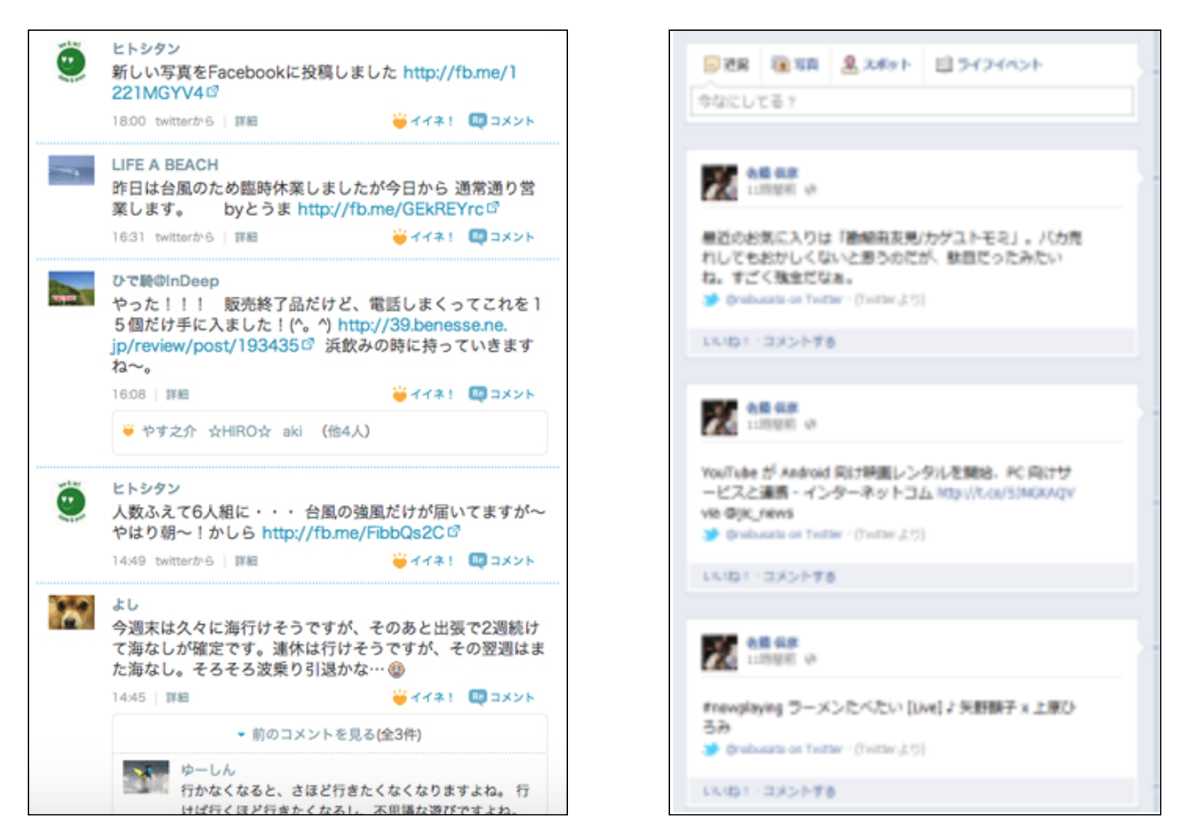
\includegraphics[width=9cm]{images/timeline.png}}
\caption{タイムライン表示}
\label{timeline}
\end{figure}

\vspace{3mm}

\paragraph*{情報ダッシュボード}

情報ダッシュボード\cite{few}は,
複数のリアルタイム情報をタイル状に並べて表示することによって
多くの情報をわかりやすく視覚化するシステムである.
たとえばWindowsのスタート画面(図\ref{windows})の情報ダッシュボードには
天気予報や株価のようなリアルタイム情報を表示可能である.

\begin{figure}[h]
\centering
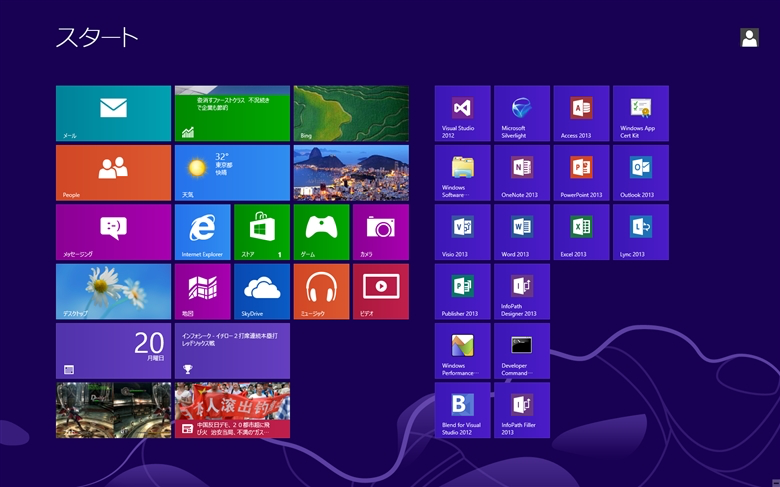
\includegraphics[width=9cm]{images/windows.png}
\caption{Windowsのスタート画面}
\label{windows}
\end{figure}

\vspace{2mm}
\paragraph*{スタンプ}

リアルタイムに流れていくタイムライン表示の中で情報を目立たせたいとき,
近年「スタンプ」と呼ばれるピクトグラムが
利用されることが多くなってきた(図\ref{linestamp}).

スタンプはテキストで記述するのが難しい表現や感情を伝えたり,
テキストを考えて入力するよりも速くて簡単であったりすることから,
近年LINEやFacebookメッセンジャー,オンラインゲームなどで広く利用されている.

\begin{figure}[H]
\centering
\fbox{
\includegraphics[width=5cm]{images/linestamp.png}}
\caption{LINEのスタンプの例}
\label{linestamp}
\end{figure}

\section{本研究の目的}
「情報ダッシュボード」の利用は広まっているが,利用できる情報の種類は限られており,
ユーザが情報を投稿して共有することはできない.
スタンプ的な表現を投稿可能な情報ダッシュボードを用意し,
その上でネット上の情報やユーザの感情/気分などを表示すれば,
現在の世界や人々の状況を一目了然に理解する(わかる)ことが可能になるであろう.
実世界の状態や人間の状況を情報ダッシュボードにわかりやすく表示し,
かつ誰もが簡単に気分などをスタンプのように投稿して共有できるシステムを開発することを目的とする.

\section{本論文の構成}

本論文は以下の8章で構成される。

第2章では、本研究の背景をより詳細に分析し、既存の視覚化システムの問題点を整理する。

第3章では、関連する研究分野についてまとめ、それぞれの利点と問題点を整理する。

第4章では、本論文で提案する視覚化システムの概要と全体像を示し、
システム全体の構成と実現すべきユーザ体験について述べる。

第5章では、本論文で提案するシステムの具体的な実装について述べる。

第6章では、本論文で提案するシステムの評価実験の概要と結果を述べる。

第7章では、第6章での結果を考察し、本論文で提案するシステムの有効性と意義について議論を行う。

最後に、第8章で本論文のまとめと結論を述べる。  % 本文1
\chapter{研究背景}
\label{chap:background}

本章では、本研究が取り扱うリアルタイム情報共有するシステムの現在の状況や情報表現の工夫について述べる。

\newpage

\section{タイムライン表示}

チャット(図\ref{chat})はインターネットを利用したテキストベースのリアルタイムコミュニケーションシステムである。
かつてはテキストを介して参加者がコミュニケーションを取るだけであったが、
現在はテキストだけでなく画像や音声などもやりとりすることができる。
チャットは数文字〜数十文字程度の文章を書き込んでやりとりすることがほとんどだが、
文字入力が間に合わず話題についていくことができなくなってしまうことがあるため、
「>」(特定の相手に対する発言)や「/」(発言の区切り)などといった記号による簡略的な表現や、
「ALL」(全員)や「ROM」(Read Only Member)などといった略語を用いて会話を行うことが多い。

また、多くのチャットのインタフェースは参加者の投稿を表示する時系列に表示するタイムライン表示を利用している。
タイムライン表示はTwitter、FacebookなどのSNSのリアルタイムのコミュニケーションや
天気予報(図\ref{weather})、株価など時間で推移する情報の表示に現在最も普及している視覚化手法である。

\begin{figure}[H]
\centering
\fbox{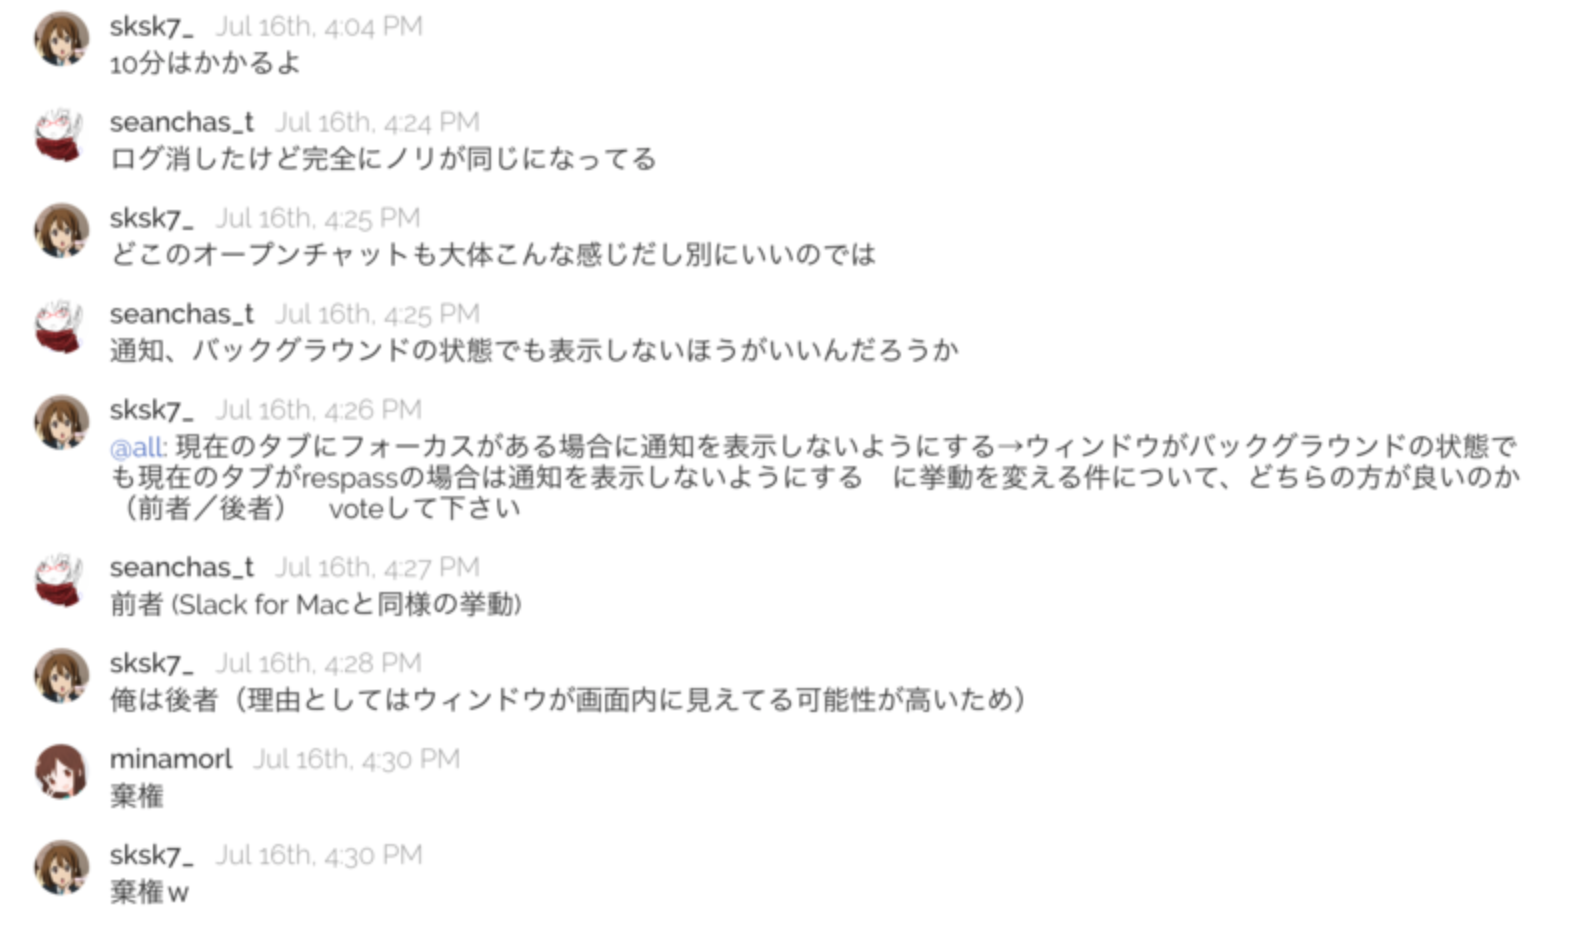
\includegraphics[width=9cm]{images/chat.png}}
\caption{一般的なテキストチャット}
\label{chat}
\end{figure}

\begin{figure}[H]
\centering
\fbox{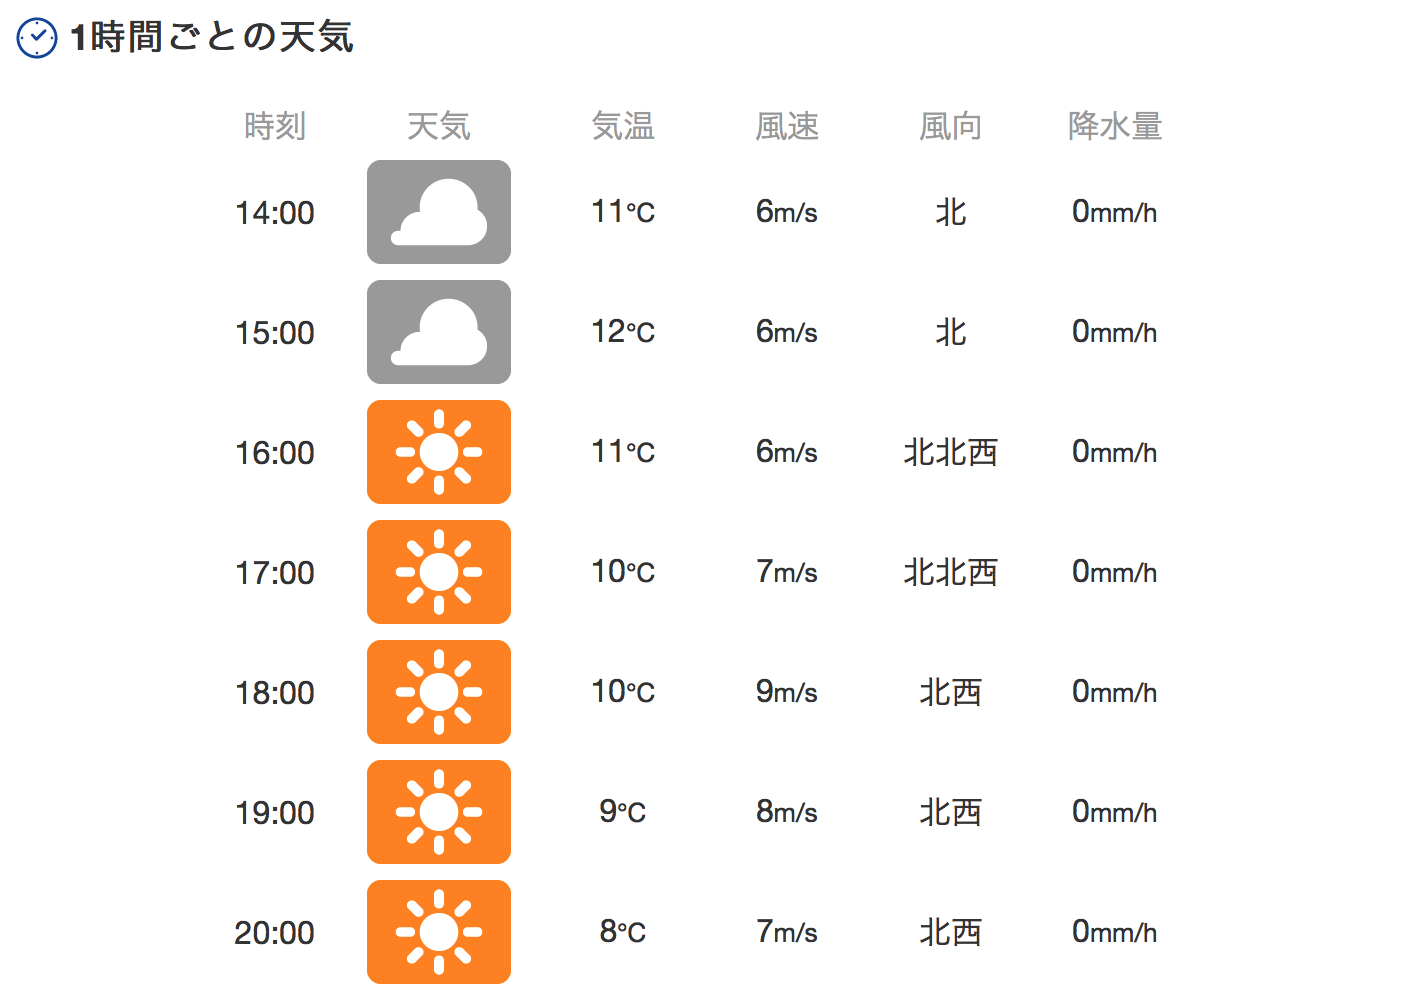
\includegraphics[width=9cm]{images/weather.png}}
\caption{時系列順に表示される天気予報}
\label{weather}
\end{figure}

日本の若者を中心に人気のコミュニケーションサービスLINE\footnote{\textsf{https://line.me/ja/}}
のトーク機能では、
テキストとは別に{\bf スタンプ}と呼ばれる大型のピクトグラムを相手に送ることができるのが特徴である。
スタンプはタイムライン表示の中で情報を目立たせたい時に使用され、
テキストで記述するのが難しい表現や感情を伝えたり,
テキストを考えて入力するよりも速くて簡単であったりすることから、
非常に便利なコミュニケーションとして浸透しつつある。
LINEは日本の20代の92.2\%が利用しているという圧倒的なシェアを誇っており\cite{soumu27}、
スタンプによるコミュニケーションもまた多くの人に利用されている\cite{40020496489}。
近年ではLINEだけではなく、Facebookメッセンジャー\footnote{\textsf{https://www.facebook.com/messages/}}
などの他のコミュニケーションサービスや、
オンラインゲームなどでもスタンプが利用されるようになっている(図\ref{gamestamp})

\begin{figure}[H]
\centering
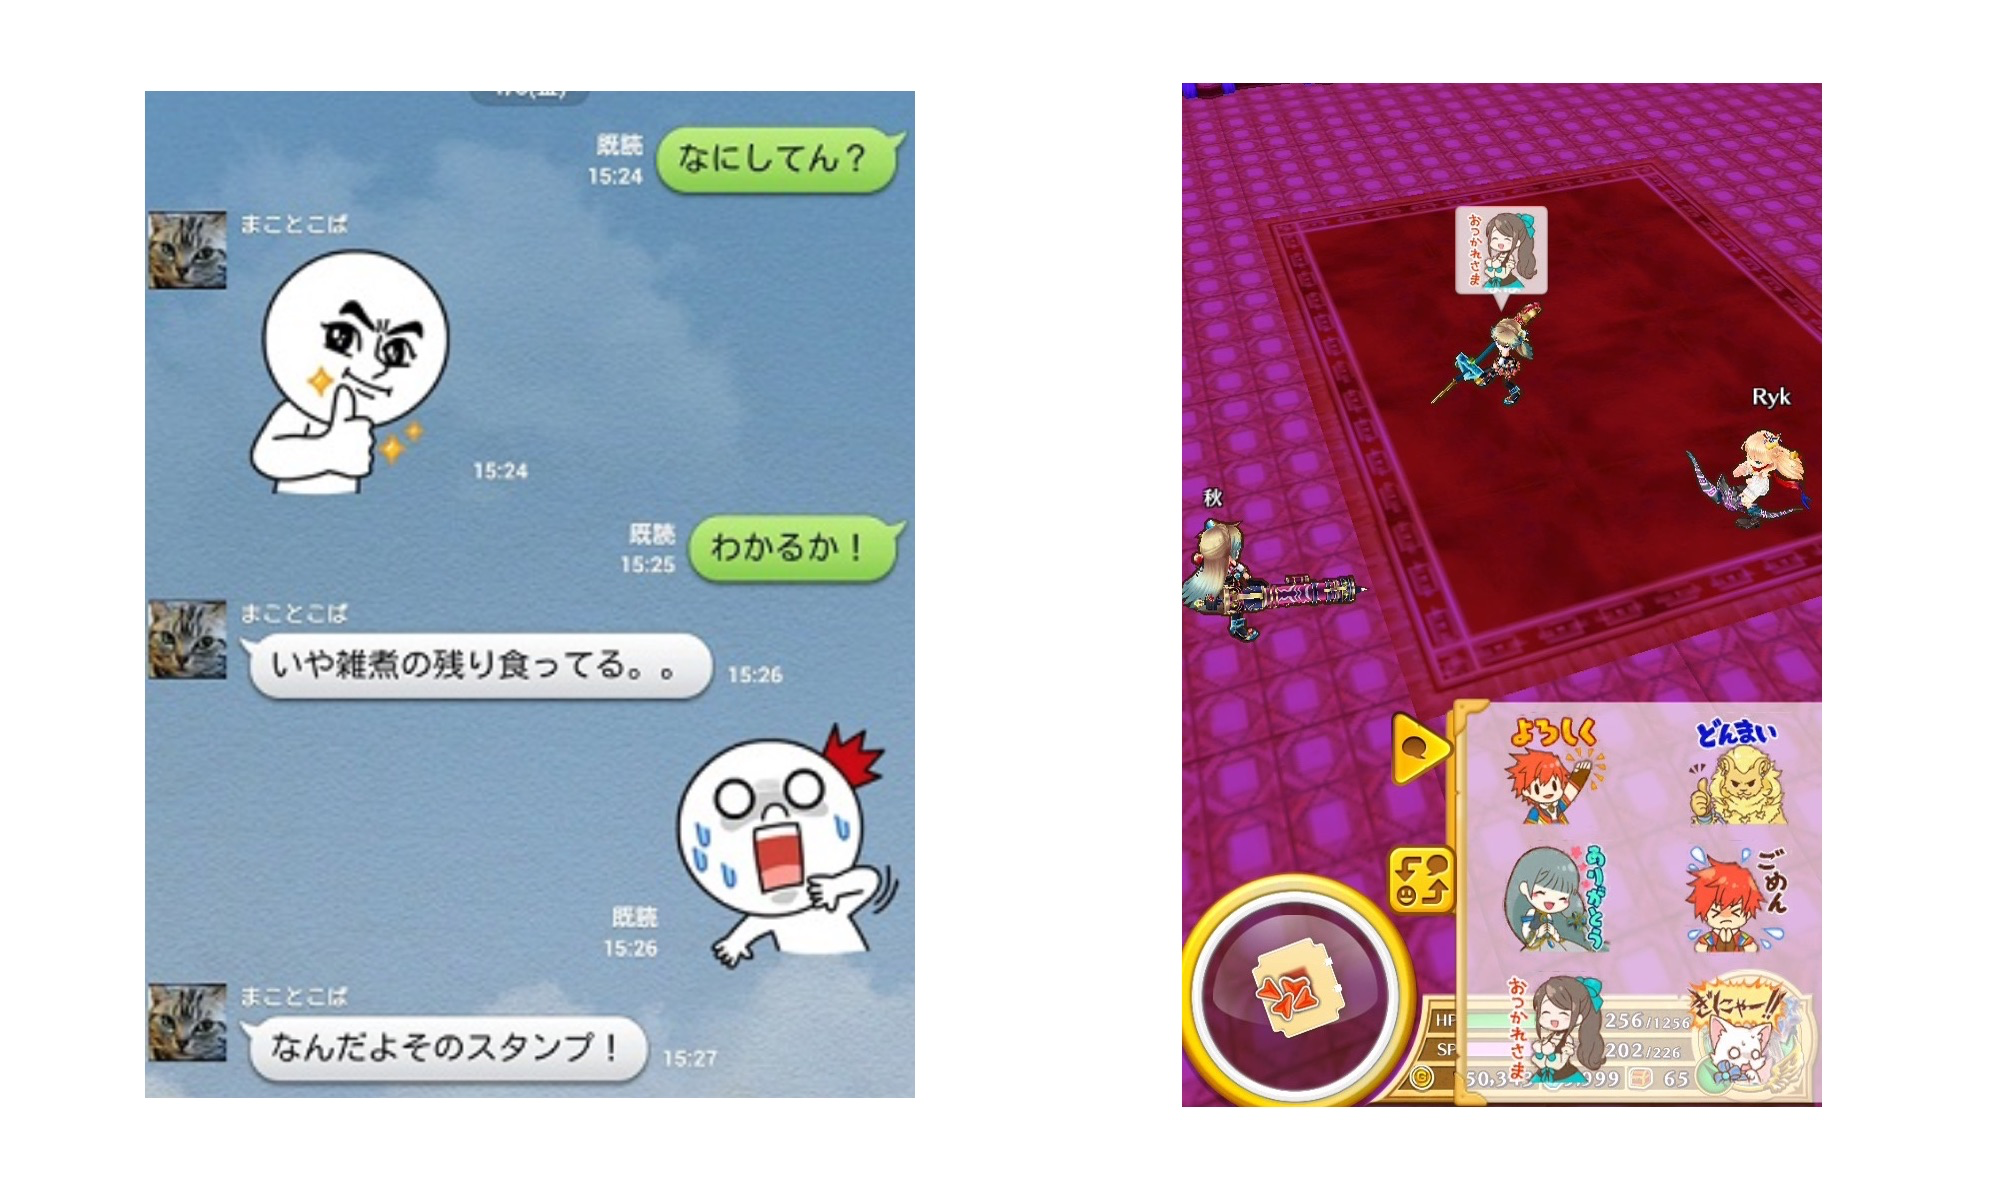
\includegraphics[width=11cm]{images/gamestamp.png}
\caption{LINEのトーク(左)とオンラインゲーム(右)で使われるスタンプ}
\label{gamestamp}
\end{figure}


\section{リアルタイムコンテンツ視聴中の情報共有}

発表や講演、テレビ放送などのリアルタイムコンテンツを視聴している際に、
他の視聴者はどのように感じたのか、知りたいことがある。
一人で視聴するよりも他の人と一緒に見た方が楽しかったり,
リビングで家族とテレビを見ながら団欒することが楽しかったりするのはそのためであり,
人と体験を共有することは重要なコミュニケーション手段である.

近年では、リアルタイムコンテンツを視聴中のコミュニケーションを行う様々なシステムが提供されている。
例えば、日本ソフトウェア科学会主催のWISS(Workshopn on Interactive Systems and Software)
コンファレンス\footnote{\textsf{http://wiss.org/}}では、
1997年から発表・聴講・議論・記録をサポートし盛り上げる新たなシステムを募集し、
会期中に実験的に運用されている\cite{wiss_challenge}。

動画投稿サイト「ニコニコ動画\footnote{http://www.nicovideo.jp}」では、
動画再生中にユーザがコメントをテキストを入力しボタンを押すことよって投稿され、投稿順に記録される。
記録されたコメントは他のユーザが同じ動画を鑑賞した場合にも反映され、
コメントが投稿された動画上のタイミングで動画上に重畳表示される(図\ref{niconico})。
コメントの投稿に時間差があっても、動画内の時間軸においては常に書き込まれた時と同じタイミングで表示されるため、
ユーザは実時間を超越した擬似的な時間共有を体感することが出来る。
これは、チャットや掲示板のような時系列に基づくメディアとは異なるユーザ体験をもたらしている\cite{110006793374}。

\begin{figure}[H]
\centering
\fbox{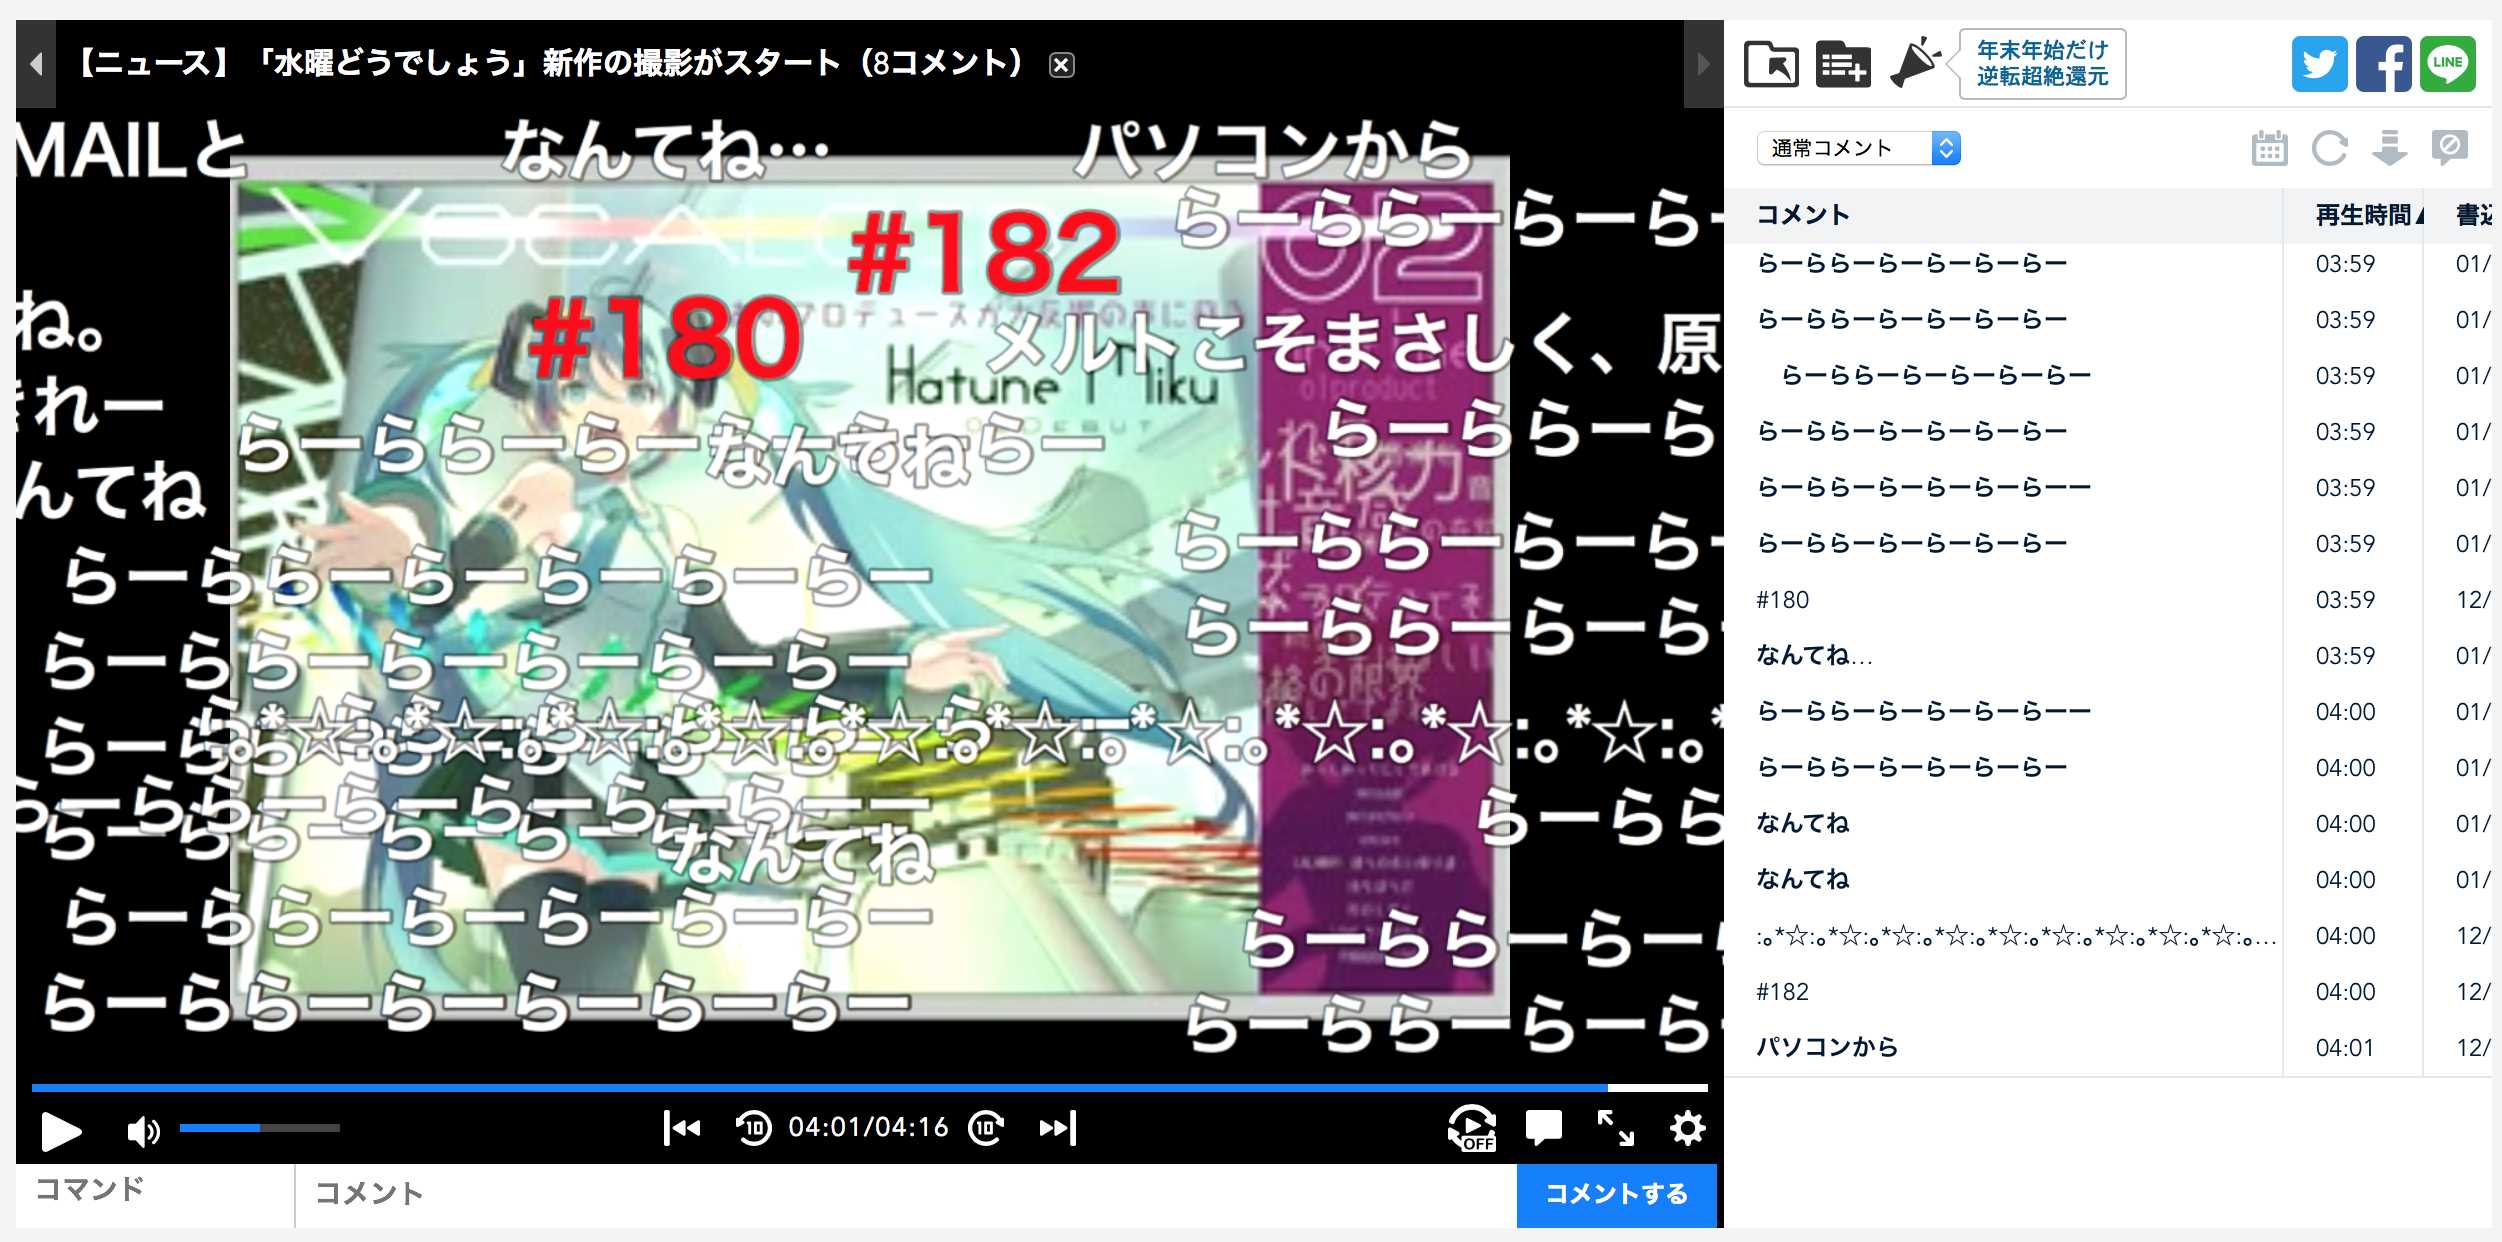
\includegraphics[width=10cm]{images/niconico.png}}
\caption{ニコニコ動画のコメント重畳表示}
\label{niconico}
\end{figure}


\section{情報ダッシュボード}

情報ダッシュボードは図\ref{azure}単一の画面に複数のリアルタイム情報を
タイル状に並べて表示するものである\cite{few}\cite{few2005}。
近年のICTやIoTなどの技術革新に伴い、センサーなどによる設備の稼動状況や
webから入手できる情報など大量の情報が溢れかえっている。
情報ダッシュボードはセンサの値や株価など常に値が変化していくものを複数並べて、
ひと目で把握するのに非常に便利なインタフェースである。
情報ダッシュボードには多くの製品やサービスが存在するが、
利用できる情報の種類は限られており、あらかじめ用意された種類の情報しか表示できない。

\begin{figure}[H]
\centering
\fbox{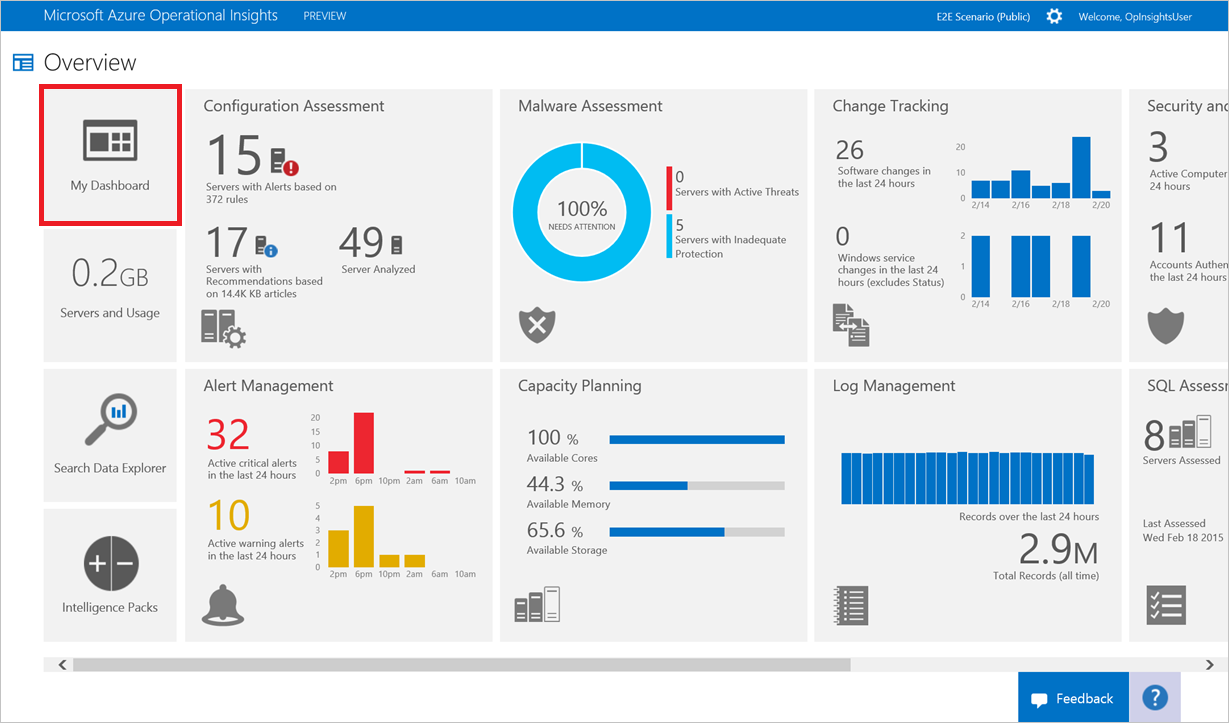
\includegraphics[width=10cm]{images/azure.png}}
\caption{Microsoft Azureの情報ダッシュボード}
\label{azure}
\end{figure}  % 本文2
\chapter{関連研究}
\label{chap:relevant}

本章では、情報ダッシュボードに関する研究と
沢山の人がいる状況での計算機を用いたコミュニケーションの支援に関する研究を紹介する。

\newpage

\section{情報ダッシュボード}

情報ダッシュボードのデザイン\cite{few}に関する研究は多くないが,
表示するべき情報を選択する手法\cite{Jones:2015:ECI:2800835.2800963}や,
セルの自動配置手法\cite{Hertzog:2015:BSP:2678025.2701383}などの
研究が存在する.

\subsection{Exist.io}
Jonesはデータ集約ツールに多面的な相関情報を提供することで生じる固有の課題について説明し、
情報ダッシュボードに表示すべき情報を選択する手法をを提案している。
また、その手法で実装されたデータ視覚化システム「Exist.io\footnote{https://exist.io}」(図\ref{existio})を紹介し、
既存のツールを改善するための設計上の考慮事項について述べている。

\begin{figure}[H]
\centering
\fbox{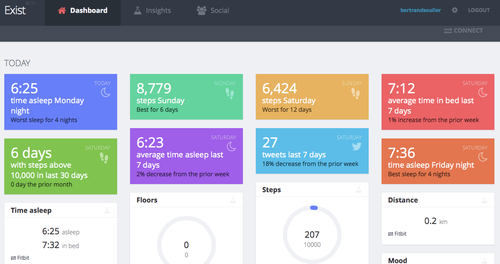
\includegraphics[width=9cm]{images/existio.png}}
\caption{Exist.io}
\label{existio}
\end{figure}

\subsection{Binary Space Partitioning Layouts}
Hertzogは情報ダッシュボードのレイアウトが柔軟性に欠けていることを指摘している\cite{Hertzog:2015:BSP:2678025.2701383}。
今日の多くの情報ダッシュボードアプリケーションはレイアウトのカスタマイズを提供しないか、
レイアウトマネージャを提供していたとしてもしてもその制御が非常に難しいことを問題としている。
そこで、バイナリ空間パーティショニング(Binary Space Partitioning)に基づいた自動レイアウト手法を提案し、
ユーザーが決めたレイアウトを尊重しながら、すべてのタイルの位置とサイズを実際に望ましいサイズに
できるだけ近くなるように計算するアルゴリズムを紹介している(図\ref{hertzog})。

『わかるらんど』のダッシュボードは
単純な形状のセルを指定どおりに並べているだけであるが,
よりわかりやすい表示のための配置手法の検討は意義があると思われる.

\begin{figure}[H]
\centering
\fbox{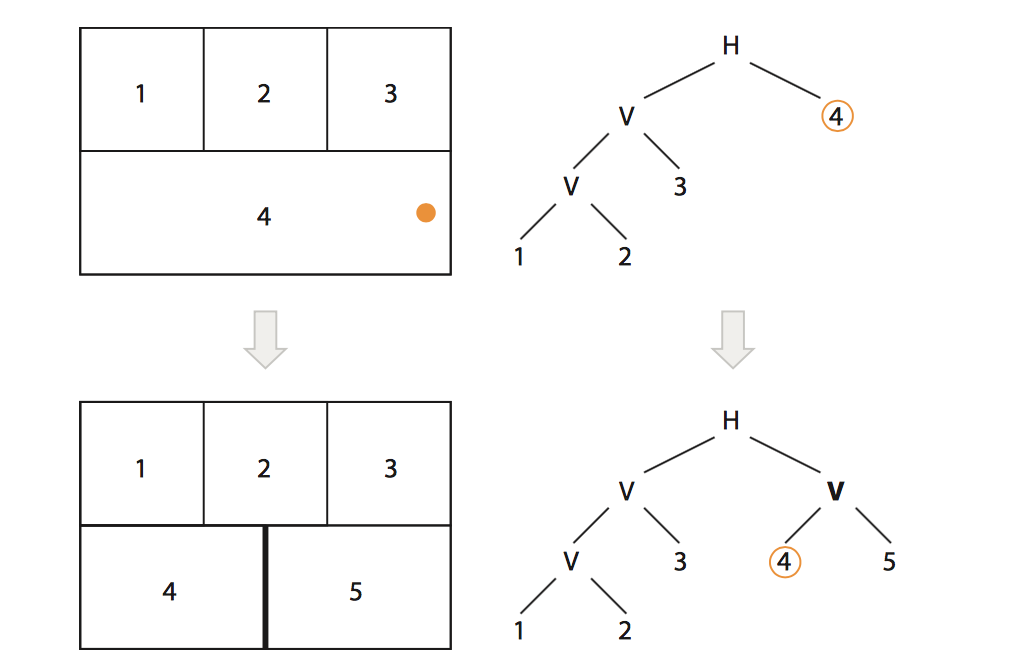
\includegraphics[width=9cm]{images/hertzog.png}}
\caption{バイナリ空間パーティショニング}
\label{hertzog}
\end{figure}


\section{沢山の人がいる状況での計算機を用いたコミュニケーションの支援}
会議での議論を促進するために
「Lock-on-Chat」\cite{nishida2006},
「On-Air Forum」\cite{nishida2011}
など様々なチャットシステムが提案されている。
このようなチャットシステムのほとんどは
タイムライン型式で表示が行なわれるようになっており,
情報ダッシュボードのような型式で感情や意見など書き込んで
一覧できるチャットシステムは存在しない.


\subsection{Lock-on-Chat}

西田らによる「Lock-on-Chat\cite{nishida2006}」(図\ref{lockonchat})は複数の話題に分散した会話を促進するチャットシステムである。
Lock-on-Chatは参加者間で画像を共有し、
それらの画像の特定部分に会話を結びつける機能が特徴である。
文書や画像と会話を結びつけるほかのシステムが,ひとつの対象について深く議論するのに適しているのに対して,
は複数の画像に分散した会話をしやすくすることに重きを置いてデザインされている.
Lock-on-Chatは学術会議 (WISS2004, 2005) において発表中に聴衆が会話するためのシステムとして運用された。

\begin{figure}[H]
\centering
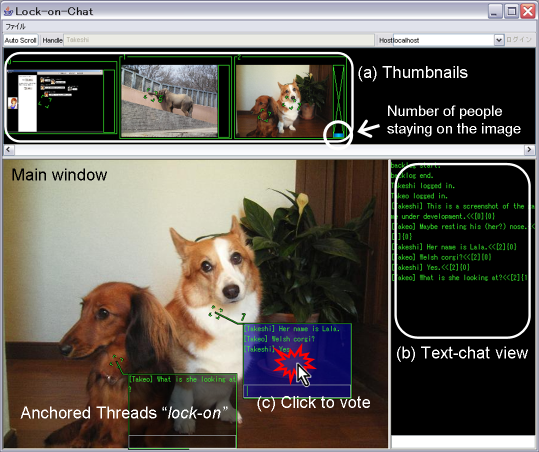
\includegraphics[width=8cm]{images/lockonchat.png}
\caption{Lock-on-Chat}
\label{lockonchat}
\end{figure}


\subsection{On-Air Forum}

西田らによる「On-Air Forum\cite{nishida2011}」(図\ref{onairforum})は
コンテンツへの没頭度合いに応じた発言の入力方法を提供するチャットシステムである。
従来のチャットシステムでは、
コンテンツとコミュニケーションを同時並行的に把握し続けるのは参加者にとっての負荷が高く,
コンテンツを視聴中の興奮やほかの発言に対する同意といった単純な反応を返すことで精いっぱいになってしまう
ことを問題としており、
コンテンツに没頭しているときでも利用できるエキサイトメッセージ機能,
テキストを入力する余裕がないときでも利用できる反応ボタンと選択肢付き発言機能を提供している。

\begin{figure}[H]
\centering
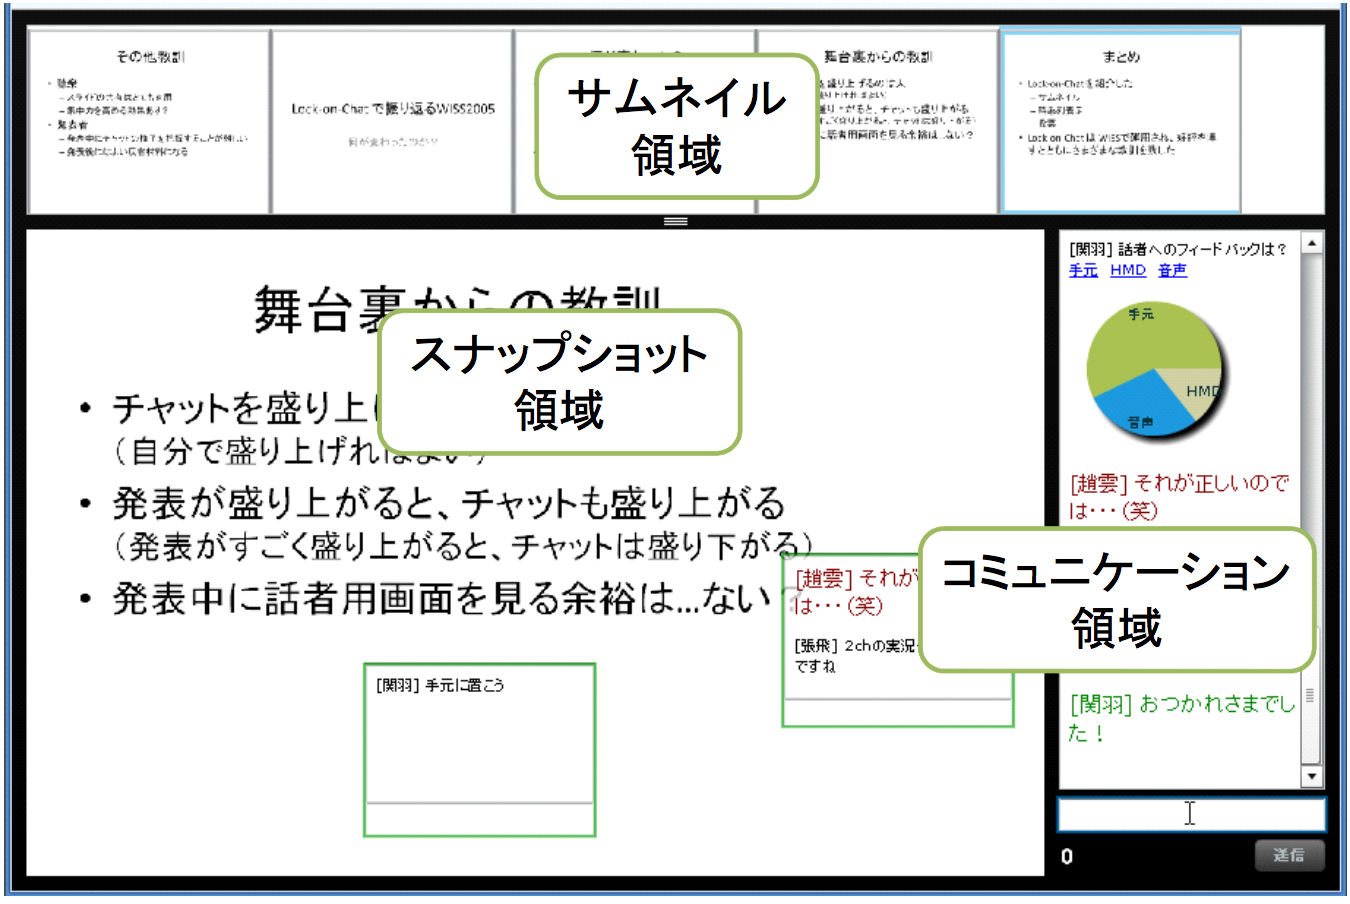
\includegraphics[width=8cm]{images/onairforum.png}
\caption{On-Air Forum}
\label{onairforum}
\end{figure}


\subsection{ラジへぇ}

加藤らの「ラジへぇ\cite{110009657336}」(図\ref{rajihe})はラジオ聴取時における感想共有システムである。
加藤らは、ラジオの「別の作業をしながらでも聴ける」という聴取スタイルに着目し,
効果音をリアルタイムに鳴らし合うことでラジオ番組に対する感想を共有するシステムを提案している。
あらかじめ用意された単純な感想をボタンを押して選択することで感想の共有を簡単にし、
音声によるフィードバックで画面を目で追えない状況でも他人の感想を知れるような工夫がなされている。

\begin{figure}[H]
\centering
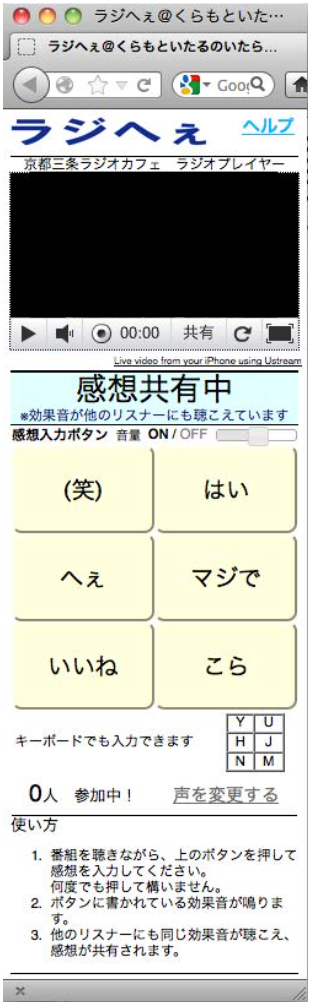
\includegraphics[width=4cm]{images/rajihe.png}
\caption{ラジへぇ}
\label{rajihe}
\end{figure}


\subsection{World Cupinion}

Shiraziらはスマートフォン上の非言語的なアイコンを用いたUIを通して
テレビ番組に関するリアルタイム意見共有システム「World Cupinion」を
提案している\cite{SahamiShirazi:2011:RNO:1978942.1978985}。
感想の投稿のインタフェースは「ラジへぇ」と同じように
あらかじめ用意された単純な感想をアイコンで表したボタンを押すことで
感想の共有をするものである。
Shiraziらは、FIFAワールドカップ2010\footnote{http://www.fifa.com/worldcup/archive/southafrica2010/}開催時に
「World Cupinion」のアプリケーションを配布して非公式な実証実験を行っており、
後から放送された番組を見返したときに、集約された感想がテレビ番組の要約に役立ったと述べている。


\begin{figure}[H]
\centering
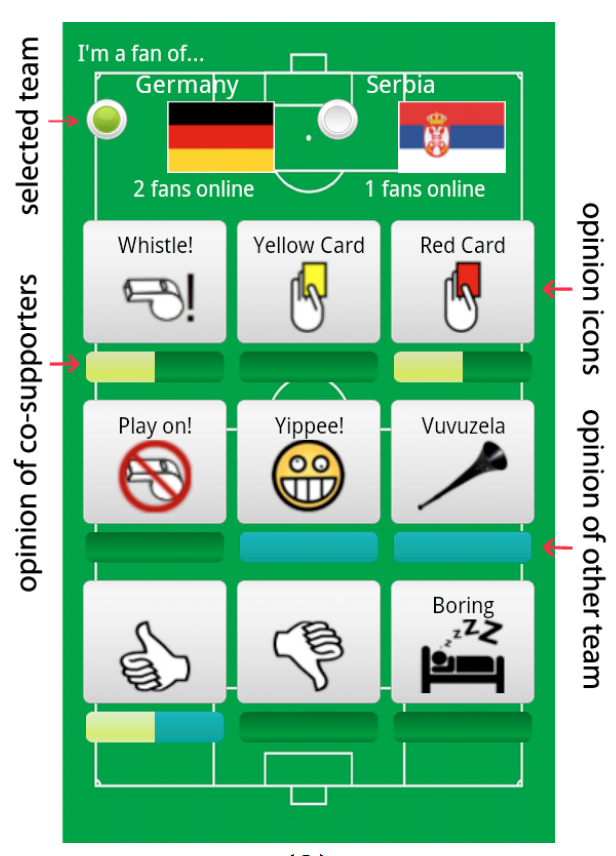
\includegraphics[width=5cm]{images/worldcupinion.png}
\caption{World Cupinion}
\label{worldcupinion}
\end{figure}


\subsection{SIGSHY}

近年,
消極的な人間でも会議の議論などに参加しやすくするための研究が
消極性研究会(SIGSHY: Special Interest Group on Shyness and Hesitation around You)
というグループなどを中心に盛んになってきているが\cite{kurihara2016}\cite{nishida2011},
本論文で提案するシステムもこのような方向性の支援に利用できると考える.  % 本文3
\chapter{設計}
\label{chap:wakaruland}

本章では,
IoT時代の情報視覚化と,
大勢の人がいる状況での計算機を用いたコミュニケーションの支援に焦点を当て,
本論文で提案する視覚化システム『わかるらんど』の設計指針と
アプリケーションのデザインについて述べる.

\newpage

\section{WISSのチャットの分析}

近年,学会などでチャットなどのコミュニケーションシステムが
利用される機会が増えていることを第\ref{chap:background_2}章で解説した.
学会チャットシステムを利用すると,
発表中に参加者が意見交換したり疑問を表明したりできるといった利点があるが,
以下のような問題も存在する.

\begin{itemize}
\item 多数の人間が同時に投稿すると投稿内容がすぐに見えなくなってしまう
\item 投稿の多いアクティブな人ばかりが目立ってしまい,消極的な参加者は議論に参加しにくい
\end{itemize}

一般に,会議などで特定の人だけが沢山発言するのはよくあることであるが,
誰もが気軽に意見を表明できる環境を構築できれば有意義であろう.

日本ソフトウェア科学会主催の
WISS(Workshopn on Interactive Systems and Software)コンファレンス\footnote{\textsf{http://wiss.org/}}では,
学会が提供するチャットシステムに参加者がログインして議論するのが恒例になっており\cite{wiss_challenge},
2009年以降のWISSコンファレンスでは「On-Air Forum」\cite{nishida2011}という学会チャットシステムが利用されている.

しかし,WISS2009の実証実験によれば,
全参加者の半分弱しかログインして1回以上発言していなかった.
またWISS2015では,252アカウントが1回以上発言し総発言数は2,948回であったが,
発言数上位20\%の50アカウントによる発言が
総発言数の78.1\%にあたる2,305回を占めていた(図\ref{wisschat}).
発言数が10回未満のアカウントは190アカウントで,これは全アカウントの75.3\%にあたる.
図\ref{powerlaw}のようにアカウントと発言数は冪分布になっており,
特定の人ばかりが発言して,発言しない人は全く発言しない傾向が顕著に現れている.

\begin{figure}[H]
\centering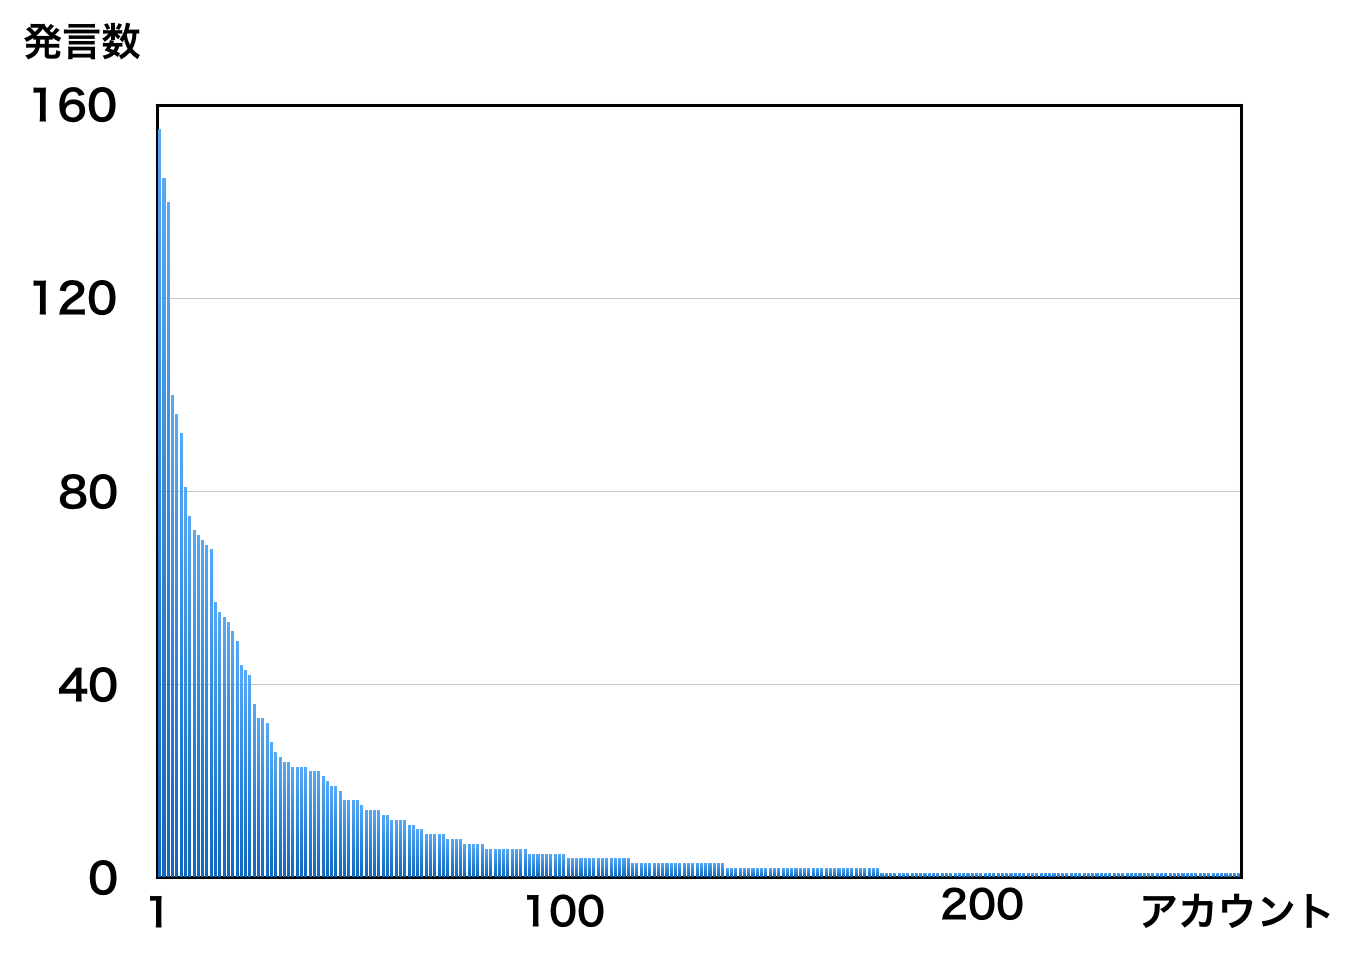
\includegraphics[width=8cm]{images/wisschat.png}
\caption{WISS2015のチャットにおけるアカウントと発言数の分布}
\label{wisschat}
\end{figure}

\begin{figure}[H]
\centering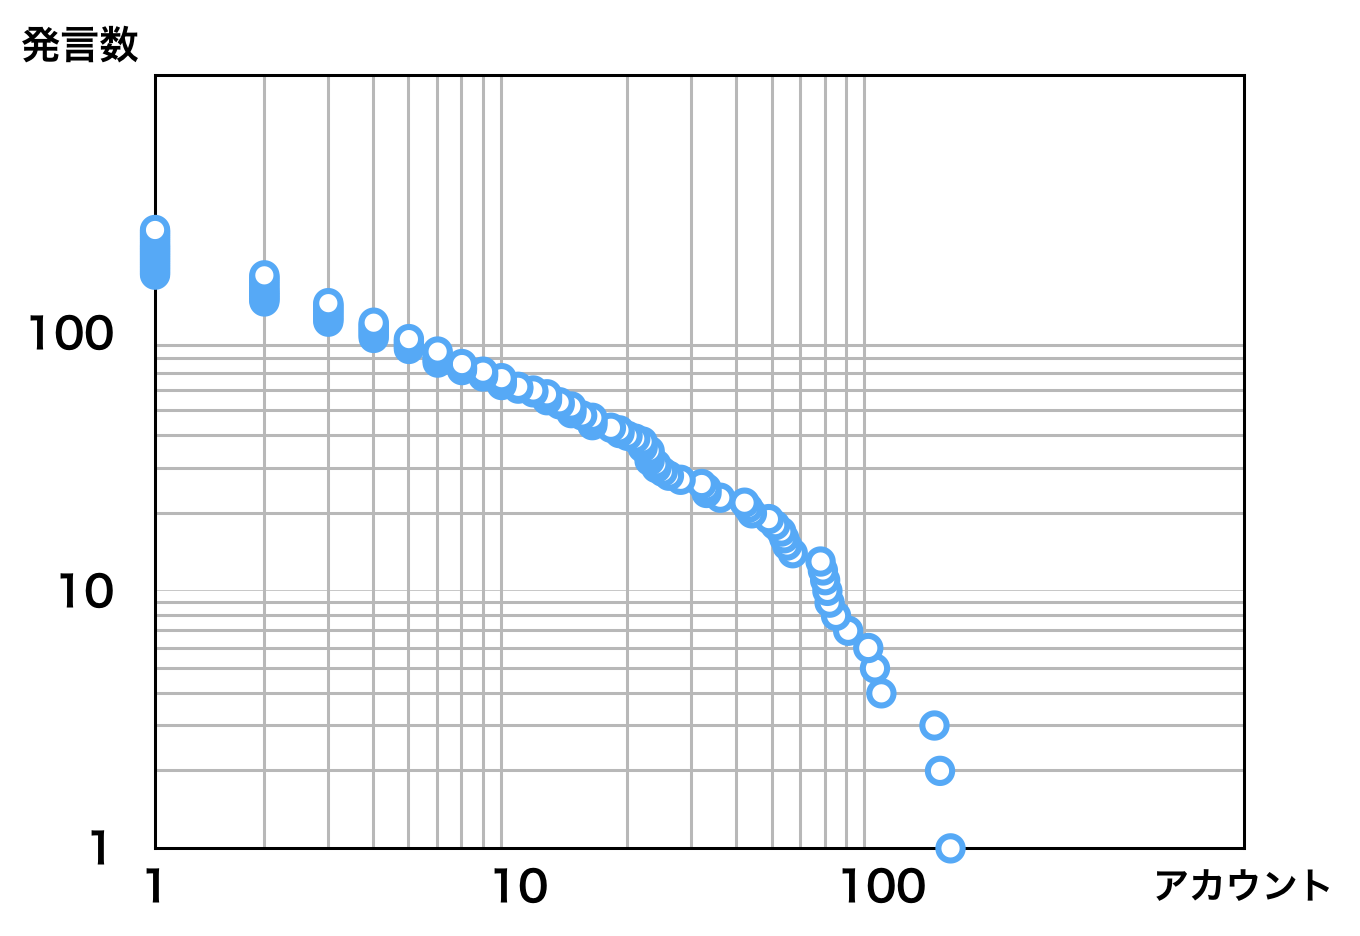
\includegraphics[width=8cm]{images/powerlaw.png}
\caption{図\ref{wisschat}の両対数グラフ}
\label{powerlaw}
\end{figure}


\section{わかるらんど}

『わかるらんど』は本論文で提案する情報視覚化システムの名称である.
『わかるらんど』では第2章で述べた視覚化システムの現状と前節で述べた問題をもとに,
単純なアーキテクチャでありながら,ありとあらゆる情報を表示可能な情報ダッシュボードを構築できる
ソフトウェアをデザインした.
本節では『わかるらんど』の主な機能とねらいについて述べる.

\subsection{ユーザインタフェース}
『わかるらんど』のユーザインタフェースは「ダッシュボード」と「投稿画面」の2つからなり,
画面右上のボタンで切り替えることができる.
図\ref{dashboard}はダッシュボードのスクリーンショットである.
ユーザが投稿したテキストやスタンプや,
各種のセンサのデータなどがリアルタイムに1つの画面に表示されている.
センサのデータなどは自動的に更新され,ユーザのリアクションは図\ref{console}の投稿画面で
ユーザ名を入力し,スタンプを一覧から選んで投稿することで
自分のアイコンの上にオーバーレイ表示される.
ユーザの投稿には表示時間が設定されており,
指定時間が経過すると自動的に投稿が取り下げられるため
いつまでも古い投稿が表示され続けてしまうということはない.
表示時間はユーザがスタンプをクリックする時間の長さで設定される.
また,投稿するスタンプは投稿画面でユーザが自由に追加/削除することができる.

\begin{figure}[H]
\centering
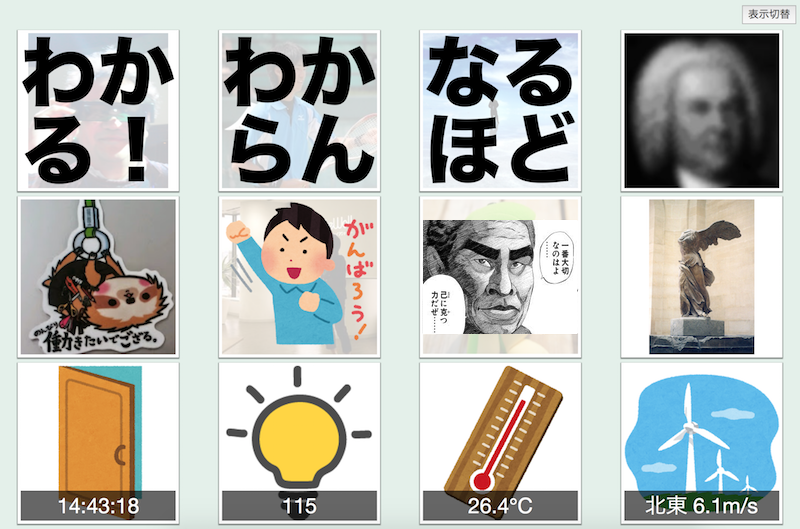
\includegraphics[width=9cm]{images/dashboard.png}
\caption{『わかるらんど』のダッシュボード}
\label{dashboard}
\end{figure}

\begin{figure}[H]
\centering
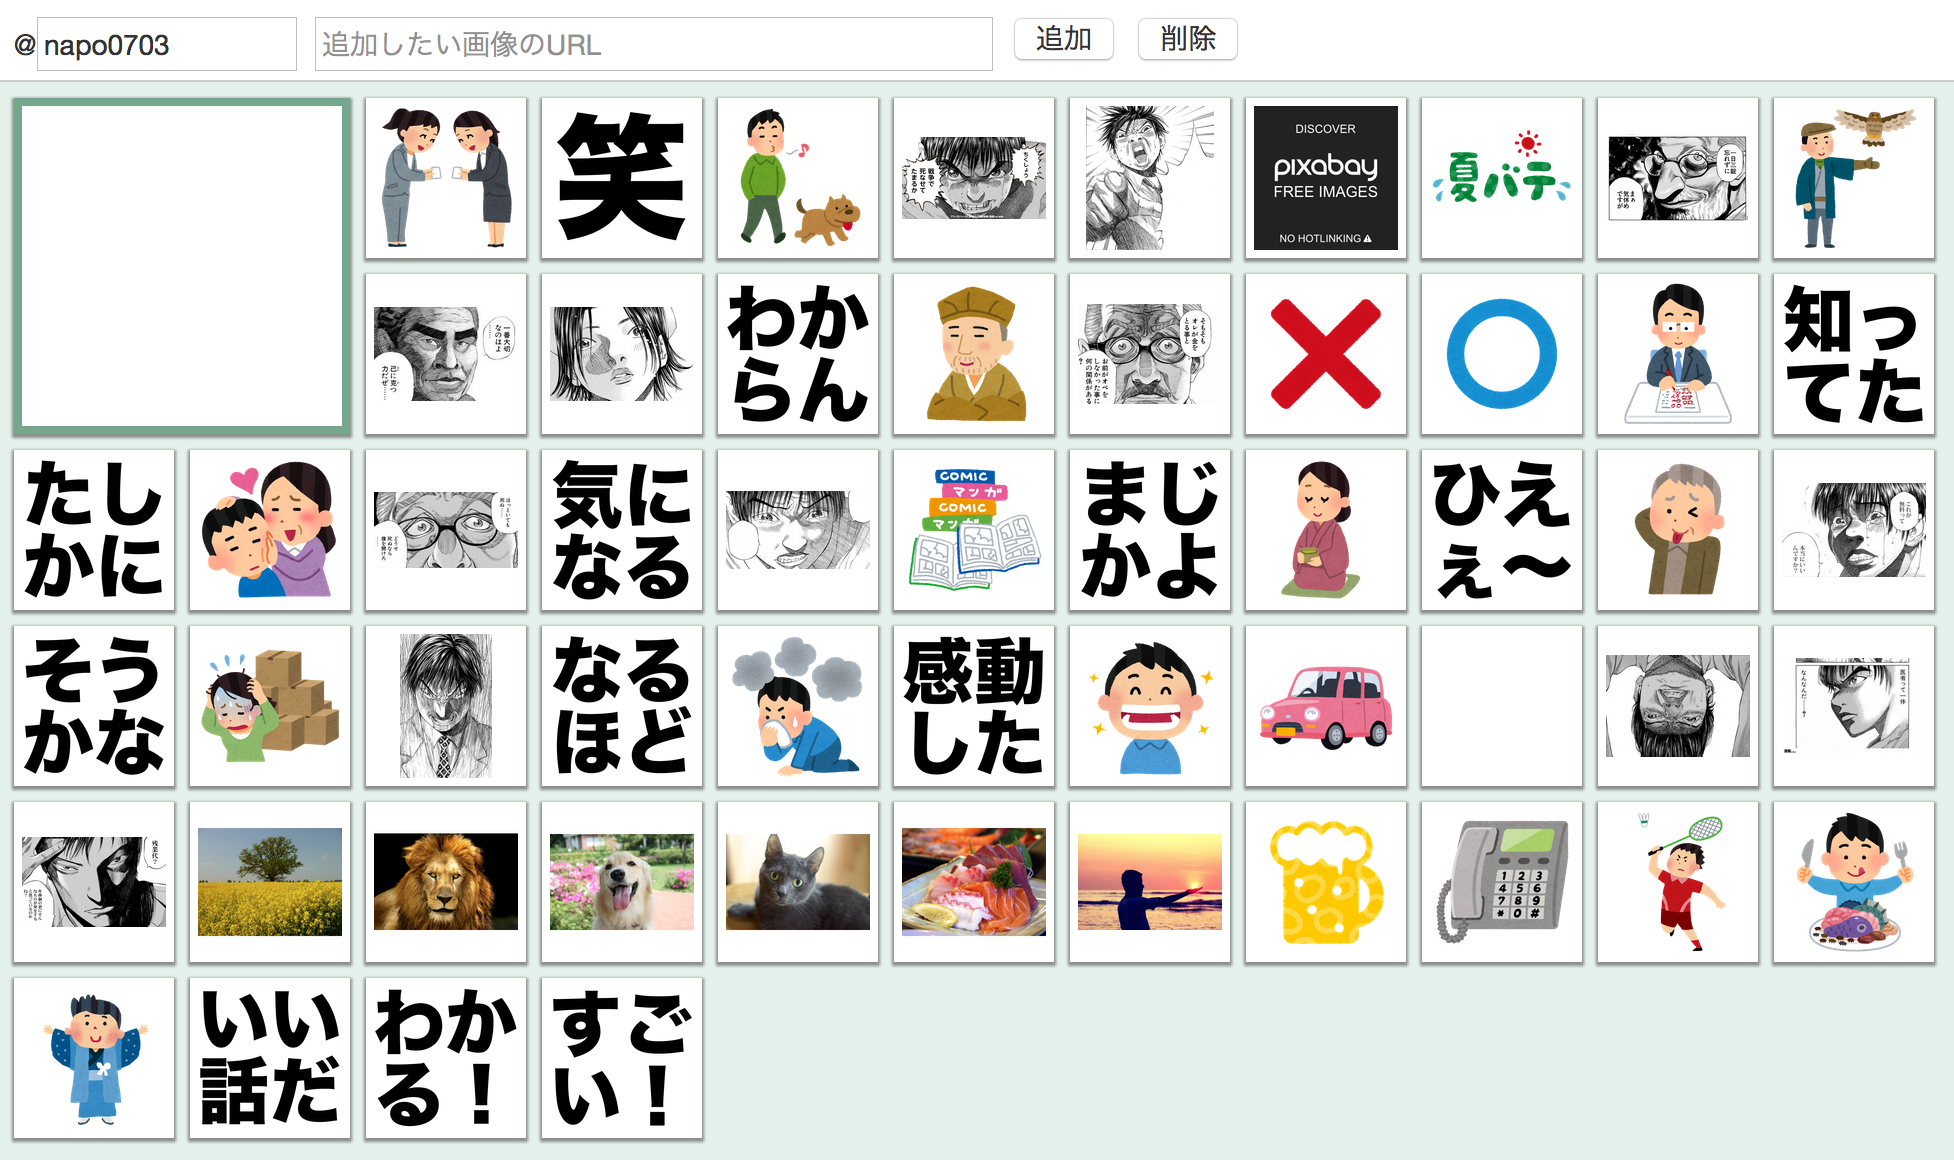
\includegraphics[width=9cm]{images/console.png}
\caption{『わかるらんど』の投稿画面}
\label{console}
\end{figure}


\subsection{表示するユーザとデータの指定}

『わかるらんど』のダッシュボードに表示されるセルは,ユーザのテキストや画像のスタンプを表示する
「リアクション」セルと,センサやWebの情報を表示する「データ」セルの2種類がある(図\ref{cell}).

\begin{figure}[H]
\centering
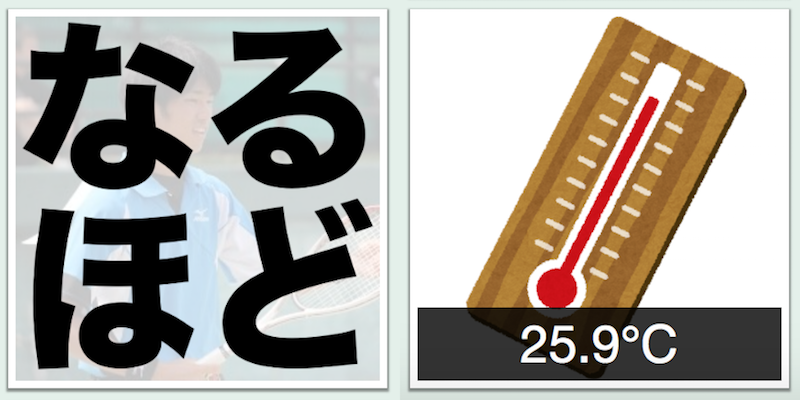
\includegraphics[width=9cm]{images/cell.png}
\caption{リアクション(左)とデータ(右)}
\label{cell}
\end{figure}

ダッシュボードに表示するユーザのリアクションの指定は,
\url{https://wakaruland.com/@napo0703,@masui,@shokai,@dorayaki0}
のようにURLの末尾にカンマ区切りでTwitterのユーザ名を「\url{@}」を付けて書くことで行う.
この場合は図\ref{n_m_s_d}のように\url{@napo0703,@masui,@shokai,@dorayaki0}の4人のユーザのセルが
ダッシュボードに表示される.

\begin{figure}[H]
\centering
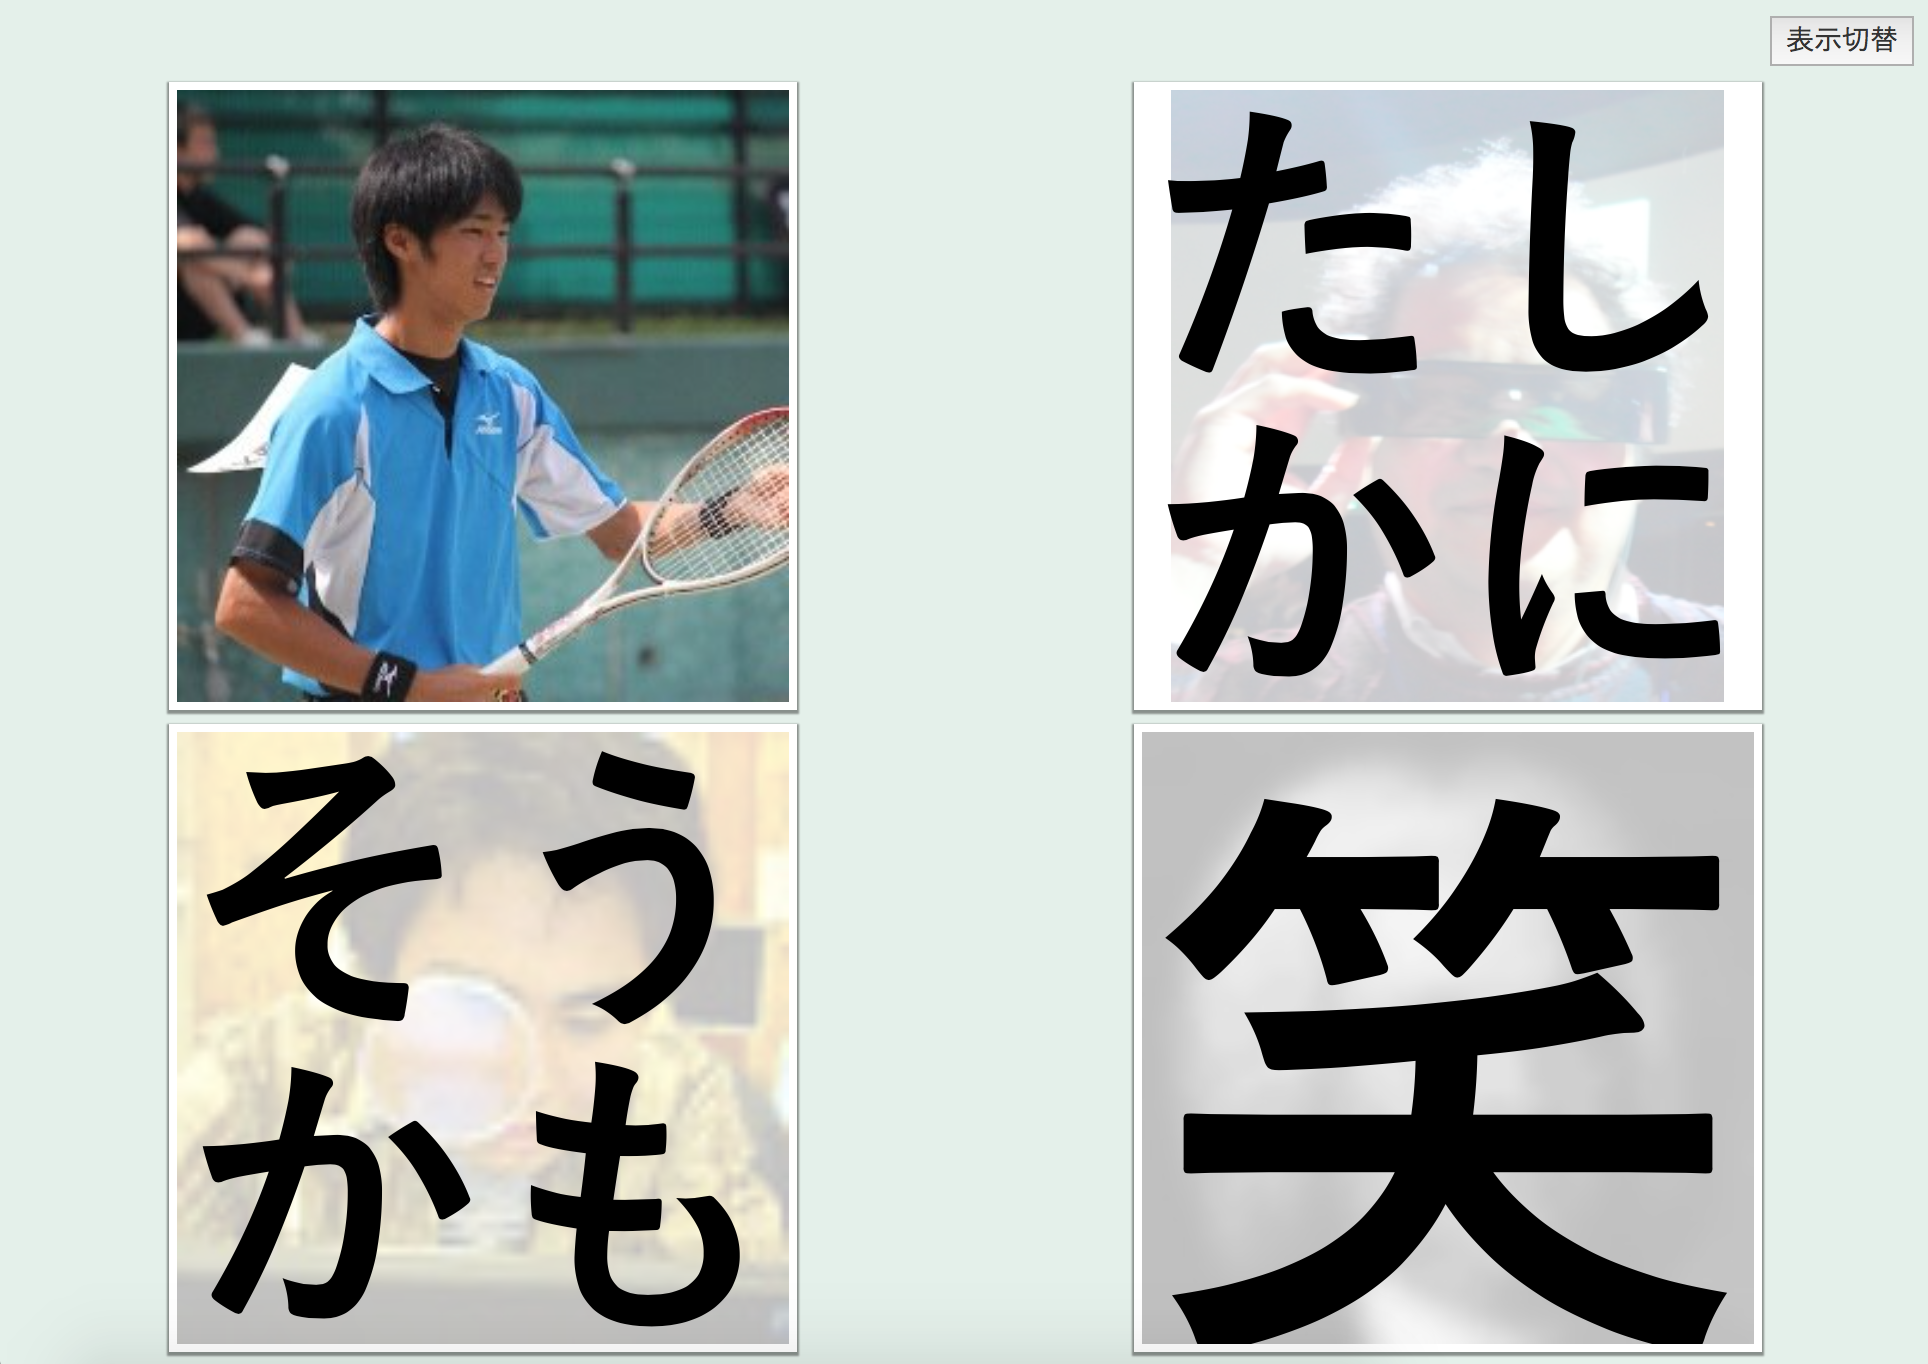
\includegraphics[width=9cm]{images/n_m_s_d.png}
\caption{4人のユーザを表示}
\label{n_m_s_d}
\end{figure}

\url{https://wakaruland.com/weather,temperature,wind}のように「\url{@}」を付けなかった場合は図\ref{w_t_w}のように\url{weather,temperature,wind}の3つがデータのセルとして表示される.

\begin{figure}[H]
\centering
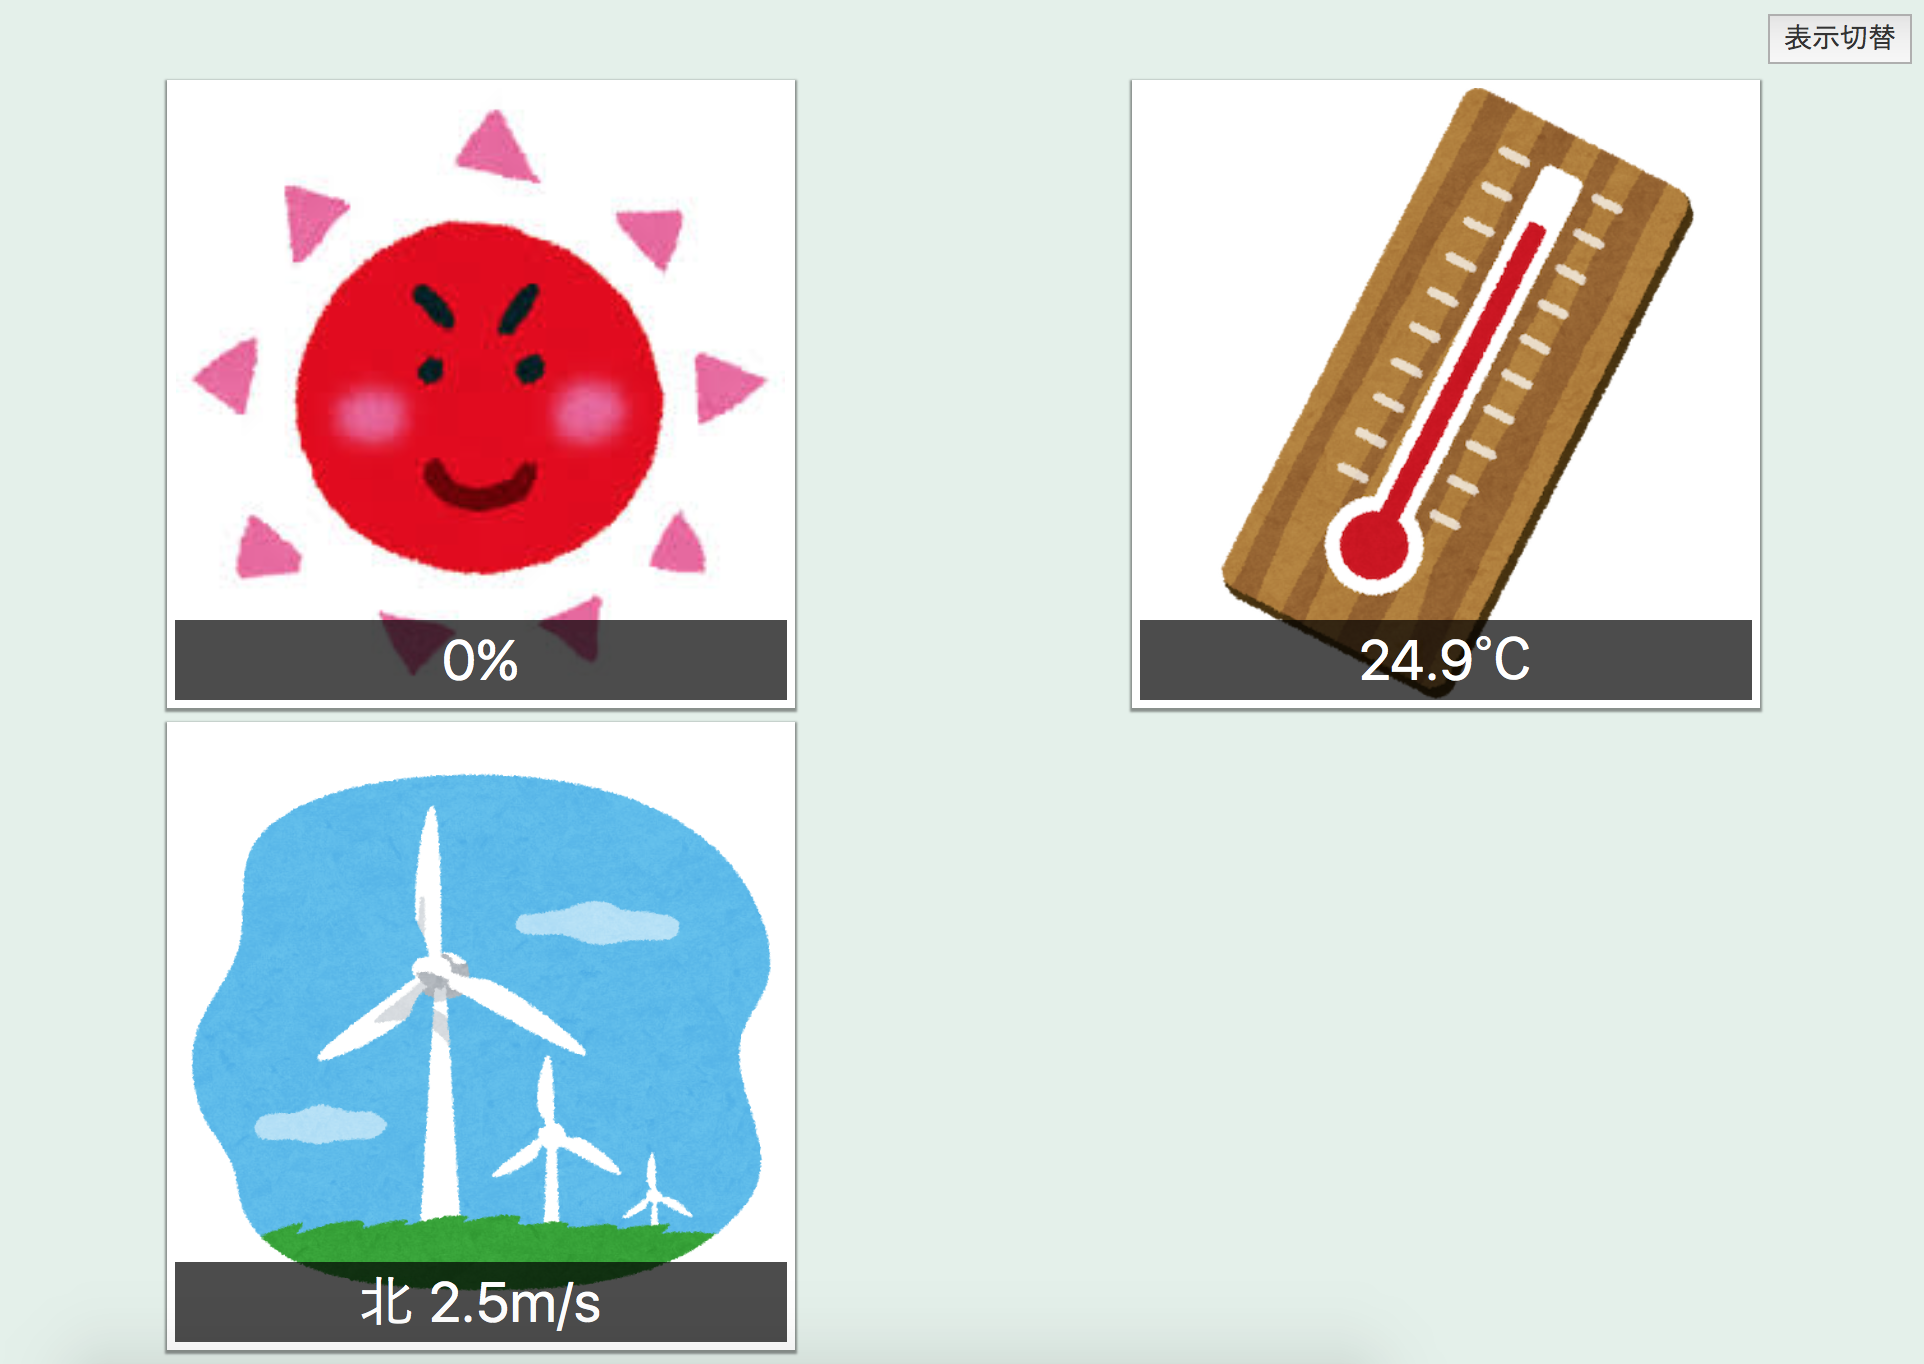
\includegraphics[width=9cm]{images/w_t_w.png}
\caption{3つのデータを表示}
\label{w_t_w}
\end{figure}

また,\url{https://wakaruland.com/@napo0703,weather,@masui,wind,@shokai}のようにリアクションとデータを合わせて表示させることも可能である(図\ref{n_w_m_w_s}).

\begin{figure}[H]
\centering
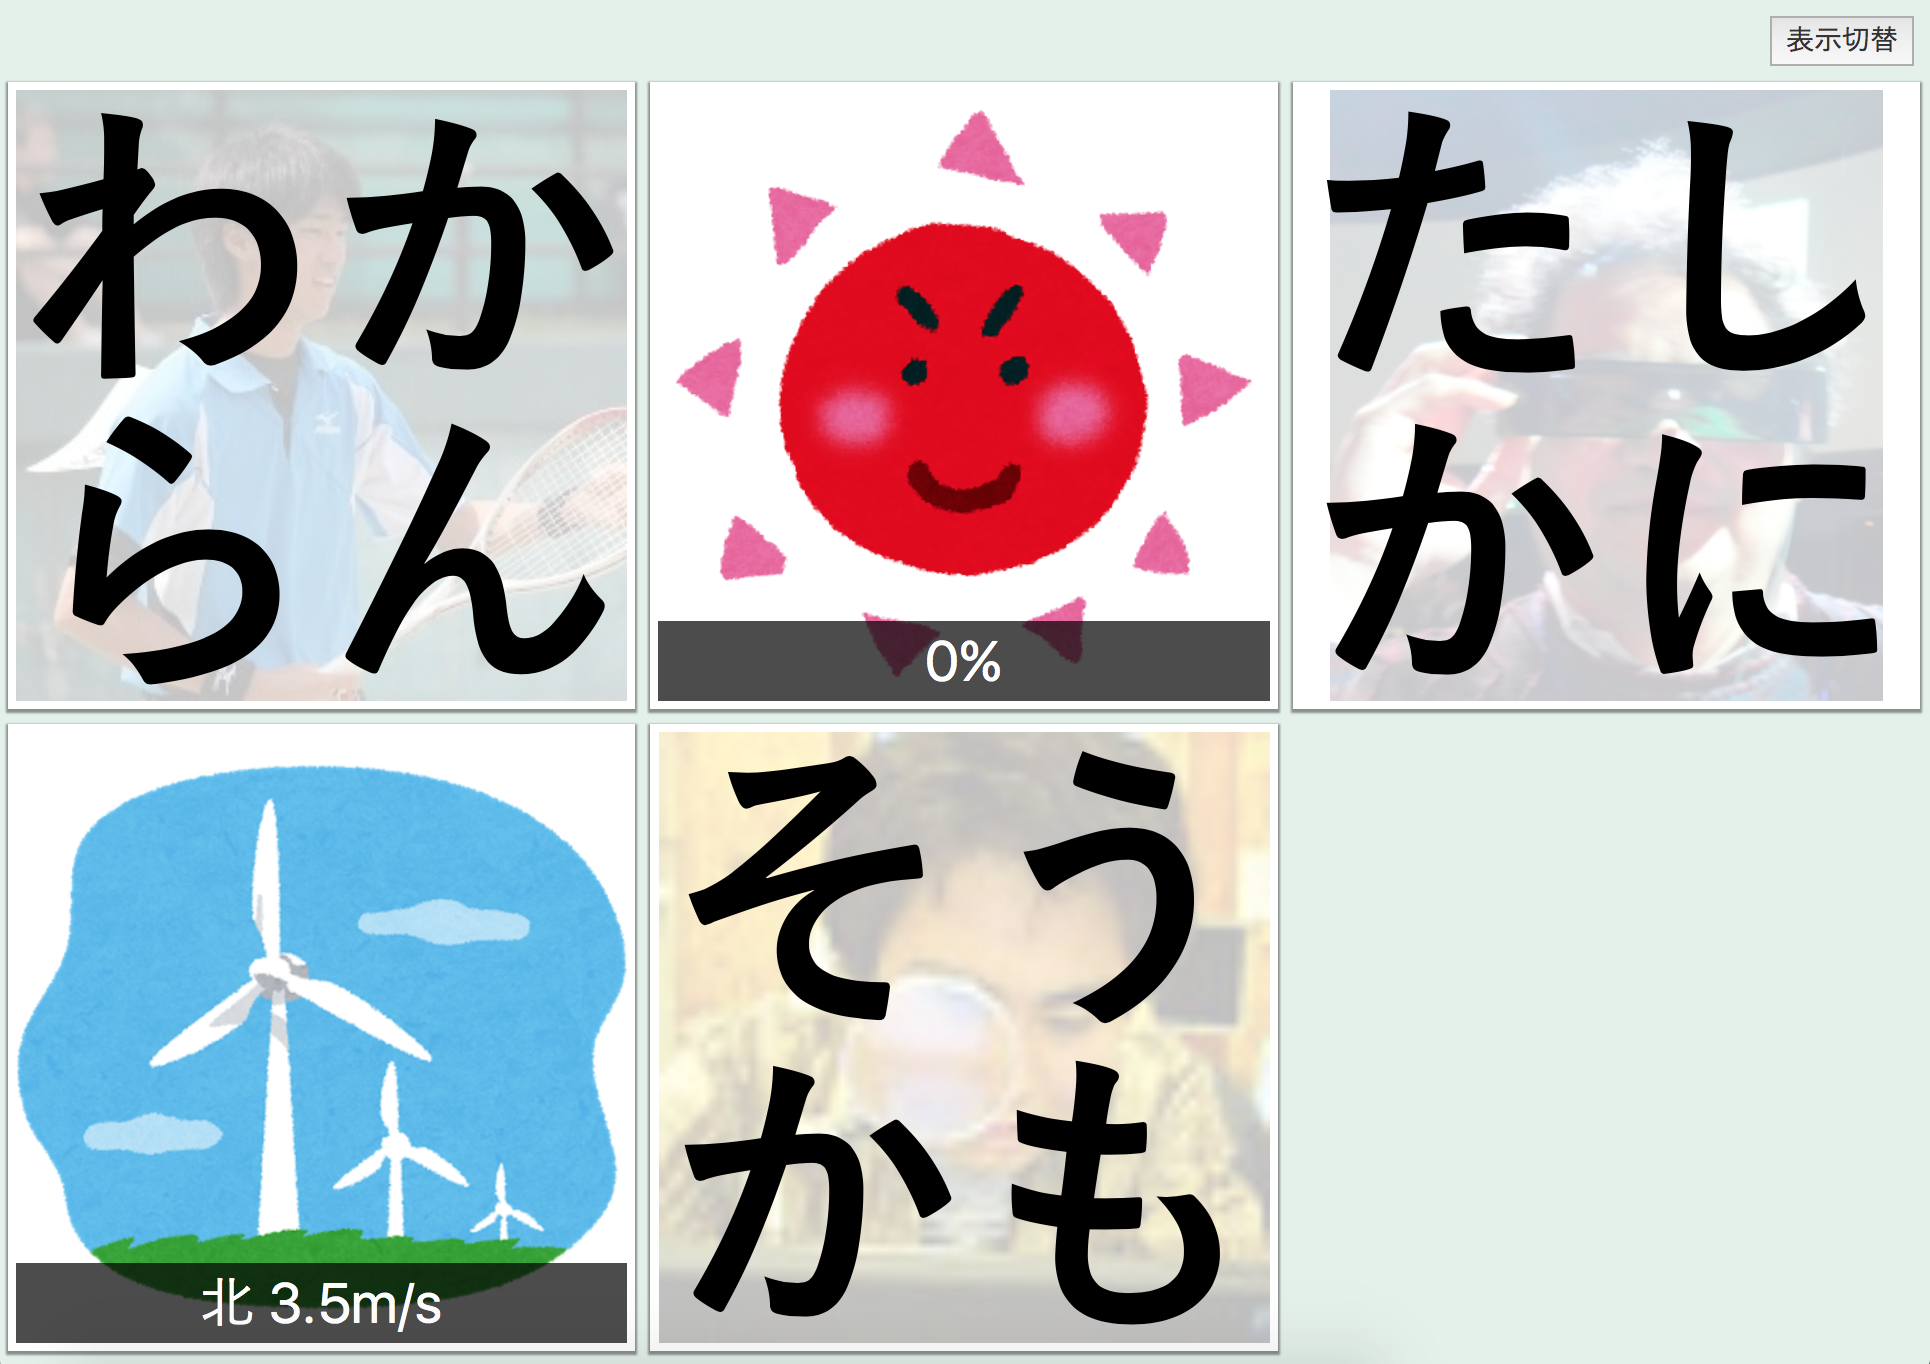
\includegraphics[width=9cm]{images/n_w_m_w_s.png}
\caption{ユーザとデータを表示}
\label{n_w_m_w_s}
\end{figure}

\subsection{スタンプの作成}
ユーザが投稿画面でリアクションとして投稿するスタンプには,
「テキスト」スタンプと「画像」スタンプの2種類がある(図\ref{stamp}).

ユーザは投稿画面のテキストボックスに文字列を入力して追加ボタンを押すことで
スタンプを作成して追加することができる.

画像スタンプは,テキストボックスに\url{http://masuilab.org/image.jpg}のようなWebにある
画像のURLを入力し追加ボタンを押すことで,URLの画像をスタンプとして一覧に追加することができる.
ローカルにある画像ファイルをスタンプとして追加したい場合は,
Gyazo\footnote{https://gyazo.com}などのアプリケーションを使って
WebにアップロードしURLを得ることで追加が可能である.

テキストスタンプは,テキストボックスにURLでないを文字列を入力し追加ボタンを押すことで作成できる.
図\ref{wakaran}左は「わからん」とテキストボックスに入力してスタンプを作成したものである.
この「わからん」は1行に表示されているが,「わか らん」と改行を入れたい場所に空白文字を入力
することで,図\ref{wakaran}右のように2行で表示される.

また,ダッシュボードには現在表示されているスタンプを自分のスタンプ一覧に追加する機能があり,
他の参加者が投稿したスタンプをコピーして使うことも可能である.

スタンプの削除は,スタンプにマウスオーバーすると右上に表示される「×」ボタンを押すことで削除できる.

\begin{figure}[H]
\centering

\includegraphics[width=9cm]{images/stamp.png}
\caption{テキストスタンプ(左)と画像スタンプ(右)}
\label{stamp}
\end{figure}

\begin{figure}[H]
\centering
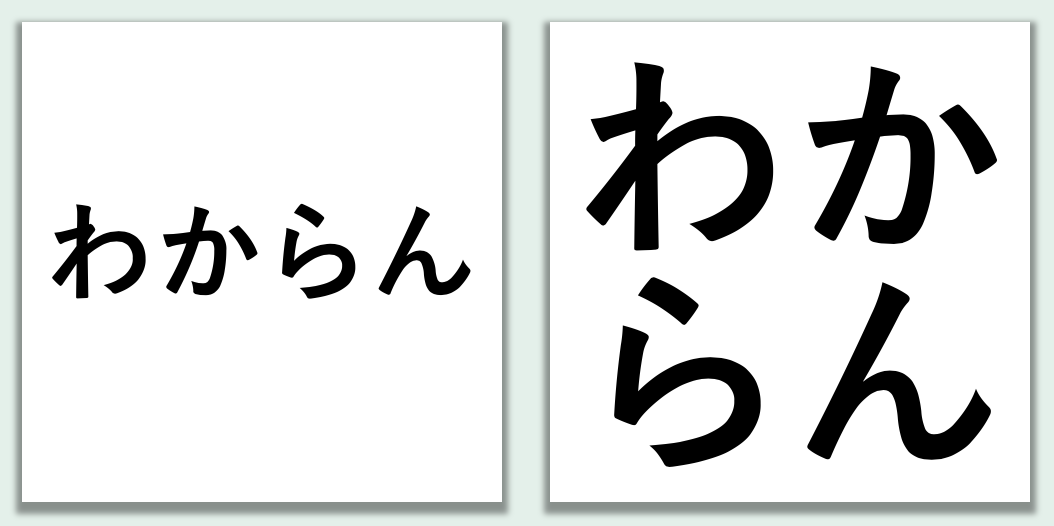
\includegraphics[width=9cm]{images/wakaran.png}
\caption{「わからん」スタンプ(左)と「わか らん」スタンプ(右)}
\label{wakaran}
\end{figure}


\subsection{利用例}
図\ref{discussion}は会議や発表の場での利用例である.
これは誰かが何か変なことを言ったのに対してユーザが反応している様子である.

図\ref{sensors}は情報ダッシュボードとしての利用例で,
各種のセンサの値やWebの情報等を表示している.
データはリアルタイムに最新のものに更新されていく.

\begin{figure}[H]
\centering
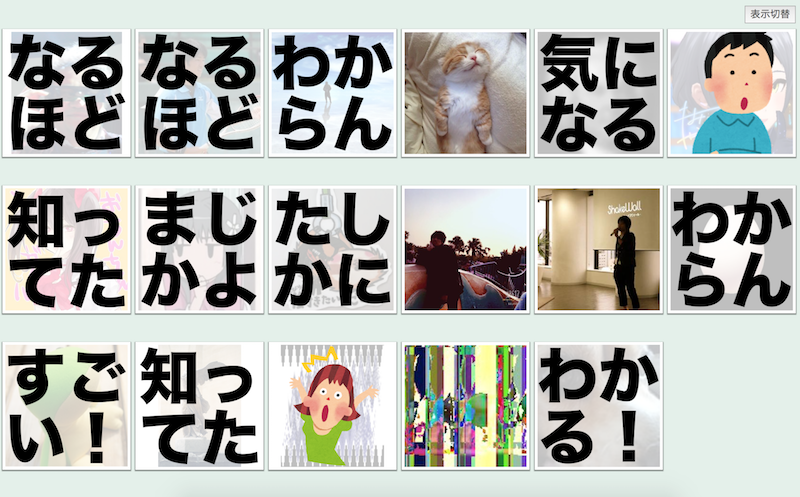
\includegraphics[width=9cm]{images/discussion.png}
\caption{会議や発表の場での利用例}
\label{discussion}
\end{figure}

\begin{figure}[H]
\centering
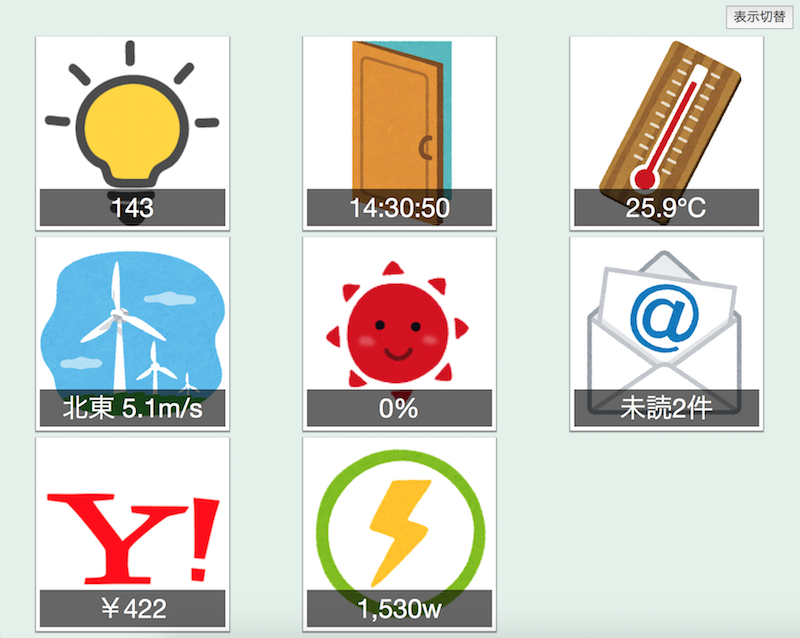
\includegraphics[width=9cm]{images/sensors.png}
\caption{ダッシュボードとしての利用例}
\label{sensors}
\end{figure}

\subsection{『わかるらんど』の情報ダッシュボードとしてのねらい}

多くの情報ダッシュボード製品/サービスが限られた情報しか表示することができないのに対し,
『わかるらんど』では適切な形でデータを用意すれば,
天気,株価,時刻などリアルタイムに流れる情報,
メールの未読件数,部屋の入退出状況などの普段通知として受け取る情報,
人間の感情や現在の状況などありとあらゆる情報を表示することができる.


\subsection{『わかるらんど』のコミュニケーションシステムとしてのねらい}
\label{nerai}

『わかるらんど』はユーザの表示領域が均等に決まっているため,
タイムライン表示のように投稿数が多い人ばかりが目立つということがない.
また,長いテキストを入力すると表示される文字が小さくなるので,
多数の人間で利用すると長い文字は小さすぎて読めない.
必然的にユーザは図\ref{wakaruland150}のように短文を入力することを強いられる.
『わかるらんど』では長文の高度な発言は期待しておらず,
「なるほど」「わからん」「笑」などといった相槌のようなものを
視覚化してひと目で把握できるようになることを期待している.
相槌は社会的承認であり\cite{130001611628},
大勢の相槌を視覚化することは大きな意義がある.
学生,教員,企業の研究者など様々なバックグラウンドの人が入り混じった状況で
「下手な発言ができない」「議論の邪魔をしてはいけない」という
投稿を躊躇させる要素を限りなく減らし,
本当は議論に参加したいけど声が出ない/手を上げる勇気がない人でも
「なるほど」「わかる」などを『わかるらんど』に投稿することで「参加」することができる.
テキストで記述すると長くなってしまう内容も
画像スタンプを投稿することで分かってもらうことができると考える.
長いテキストを投稿するには適していないので『わかるらんど』を使って議論することは難しいが,
多くの会議やコンファレンスでは発表後に議論の時間が設けられているため議論はその時に行えばよい.

\begin{figure}[H]
\centering
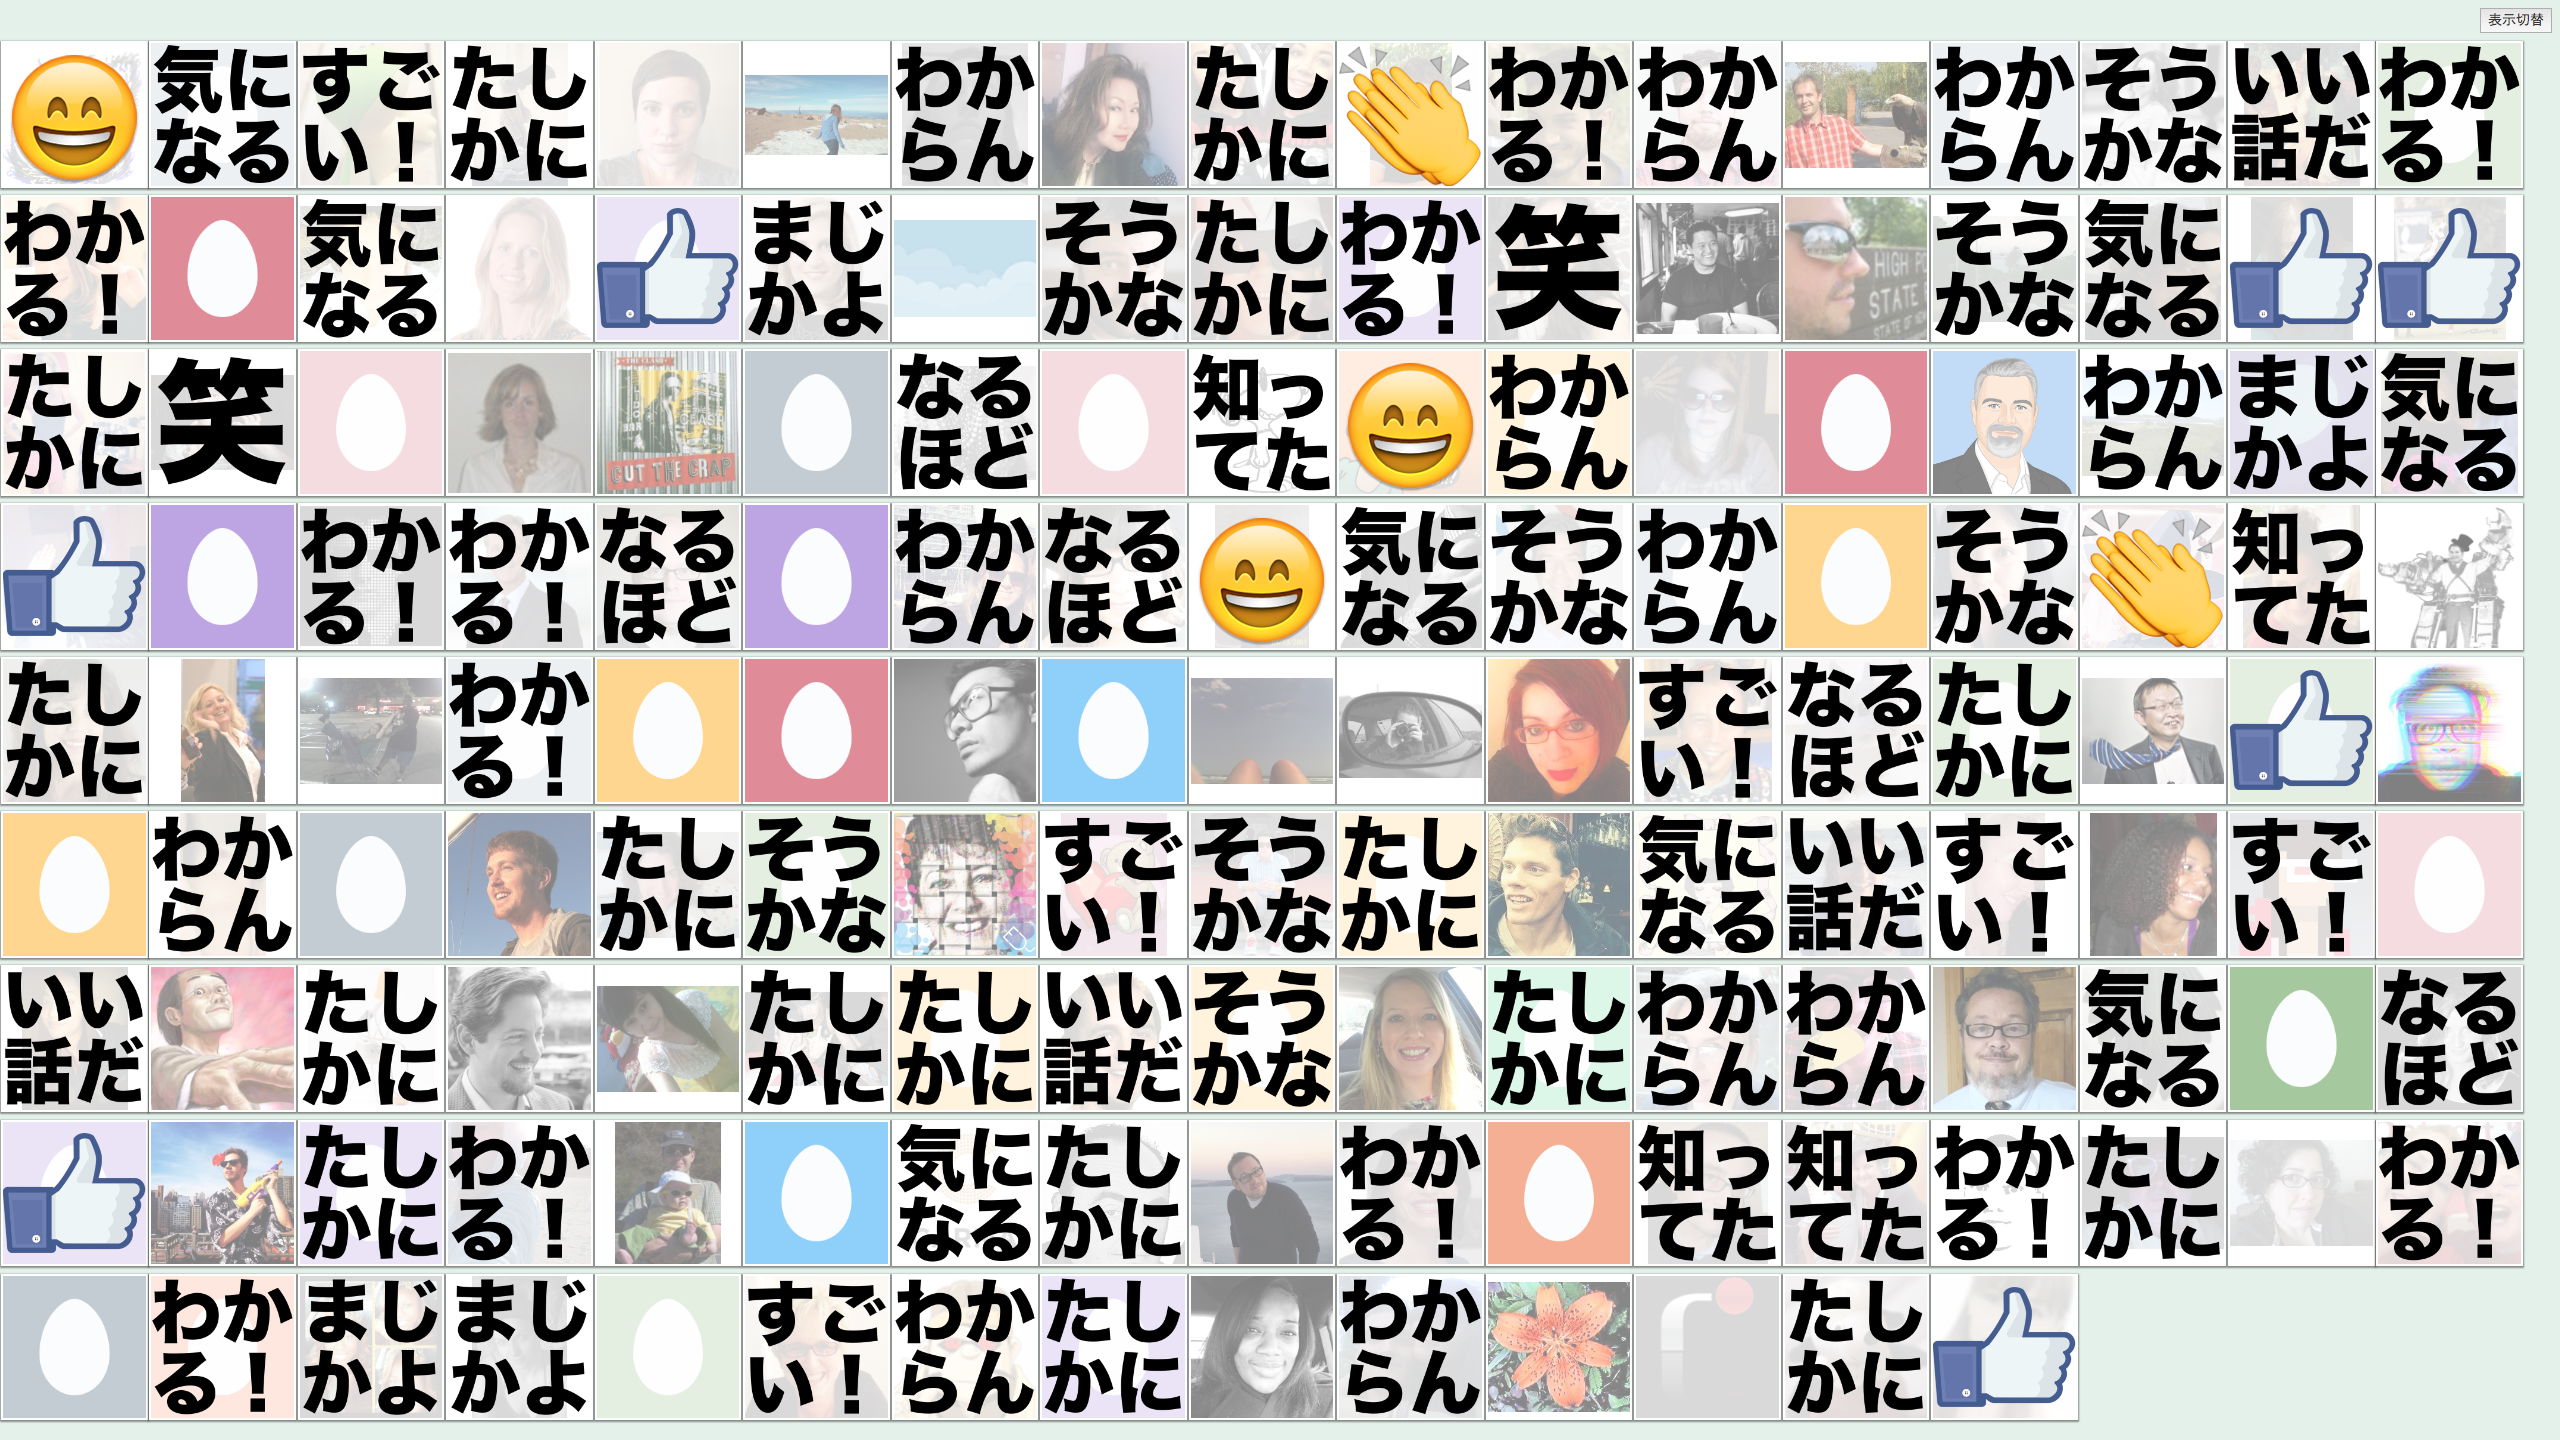
\includegraphics[width=12cm]{images/wakaruland150.png}
\caption{150人で『わかるらんど』を使用したイメージ}
\label{wakaruland150}
\end{figure}  % 本文4
\chapter{実装}
\label{chap:implementation}

本章では、第3章で述べたシステムの設計を受け、『わかるらんど』の実装について述べる。

\newpage

\section{アプリケーション構成}

『わかるらんど』のクライアントはHTML/CSS/JavaScriptで実装されており,
通常のブラウザ上のWebアプリケーションとして動作する.
サーバは,並列計算プリミティブである
\textit{Linda}\cite{Carriero:1989:LC:63334.63337}を
Webサーバ上に実装した
\textit{WebLinda}\cite{shokai_furnitue}\footnote{https://github.com/node-linda/linda}を用いて実装している.

\section{Linda}

\textit{Linda}は,
複数のプロセスで共有される空間を用いて
プロセス間通信やデータ共有をサポートする
分散並列処理を行うためのモデルである\cite{masui_linda}.
プロセスが共有する空間は\textbf{タプル空間} (Tuple Space) と呼ばれ,
タプル空間内のデータ (Tuple)を使って通信やデータ共有を行う(図\ref{linda}).
\textit{Linda}のモデルはきわめて単純であるが,
各クライアントやデバイス間で直接送信をする処理を記述する必要がなく,
柔軟で強力なプロセス間通信を容易に記述することができる.

\begin{figure}[h]
\centering
\fbox{
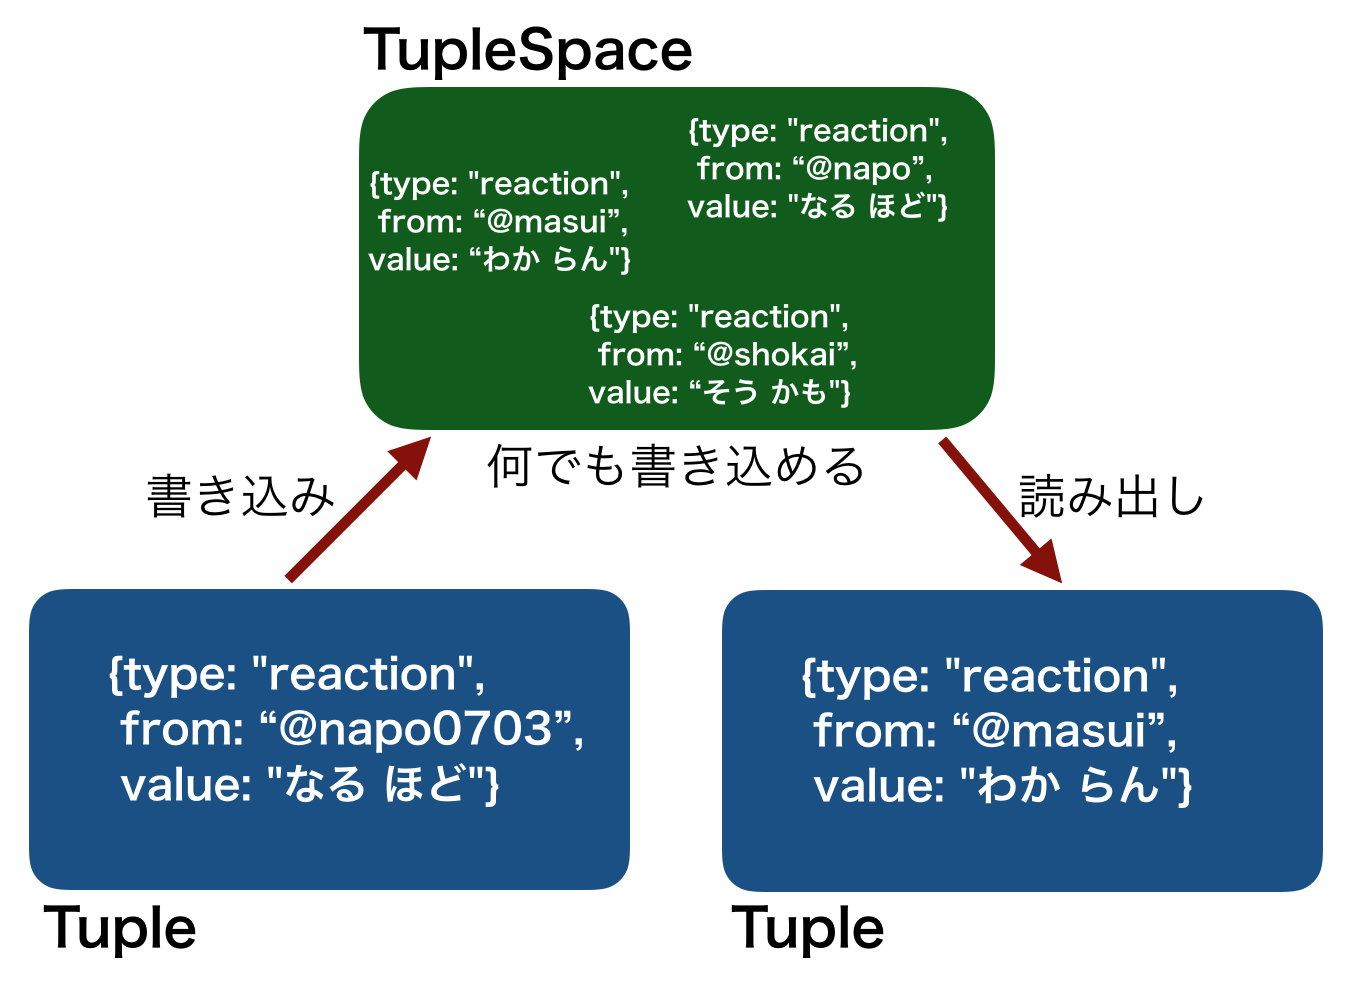
\includegraphics[width=9cm]{images/linda.png}
}
\caption{タプル空間を利用したプロセス間通信}
\label{linda}
\end{figure}

\section{WebLinda}

\textit{WebLinda}は,橋本翔氏が開発したオープンソースソフトウェアで,
Node.js\footnote{https://nodejs.org}の
WebSocketライブラリ「Socket.IO\footnote{http://socket.io}」で
実装されている.
\textit{WebLinda}は通常のWebサーバ上に実装されているため,
HTTP通信をサポートする様々な環境やプログラミング言語で利用可能である.
それゆえ,Arduino\footnote{https://www.arduino.cc}や
Raspberry Pi\footnote{https://www.raspberrypi.org}
などといった各種のIoT機器との連携も容易である.

\textit{WebLinda}は,\texttt{write}, \texttt{read}, \texttt{take}, \texttt{watch}という
4つの基本操作によってプロセス間通信を行う.

\vspace{2mm}
\begin{description}
\item[\texttt{write}]\mbox{}\\
新しいデータオブジェクト(タプル)を生成し共有空間(タプル空間)に書き込む.
\item[\texttt{read}]\mbox{}\\
タプル空間からタプルを読み出す.
\item[\texttt{take}]\mbox{}\\
\texttt{read}しつつ,読み出したタプルをタプル空間から削除する.
\item[\texttt{watch}]\mbox{}\\
タプル空間を監視し,一致するタプルが
\texttt{write}された瞬間に読み出す.
\end{description}

\section{WebLindaによる『わかるらんど』の実装}

『わかるらんど』での\textit{WebLinda}実装について述べる.
ユーザのリアクションを投稿/表示する際には,
センサと『わかるらんど』の間で

\vspace{4mm}
\begin{lstlisting}
{
    type: "reaction",
    from: "@napo0703",
    display: "60",
    value: "なる ほど"
}
\end{lstlisting}
というようなタプルをやりとりしている.

センサやWebのデータを投稿/表示する際には,
\vspace{4mm}
\begin{lstlisting}
{
    type: "data",
    from: "明るさ",
    display: "60",
    value: "500",
    background: "http://masuilab.org/image.jpg"
}
\end{lstlisting}
というようなタプルをやりとりしている.

\vspace{4mm}
\begin{description}
\item[\texttt{type}]\mbox{}\\
ユーザのリアクションの場合は\texttt{reaction},
データの場合は\texttt{data}を値にする.

\item[\texttt{from}]\mbox{}\\
投稿元を表す値.

\item[\texttt{display}]\mbox{}\\
リアクションやデータの表示時間.単位は秒.
リアクションやデータが表示されてからこの秒数が経過すると,自動的に取り下げられ表示されなくなる.
20〜86400の間で指定が可能.

\item[\texttt{value}]\mbox{}\\
リアクションの場合,この値がWebにある画像ファイルのURLだった時は,その画像を投稿者のセルにオーバーレイ表示する.
URLでない文字列の場合は,その文字列を投稿者のセルにオーバーレイ表示する.
データの場合,この値がそのままセルの下部に表示される.

\item[\texttt{background}(データのみ)]\mbox{}\\
データセルの背景画像のURL.そのデータが何を表すものなのか分かる画像を表示する.
\end{description}
\vspace{4mm}

以下は,ボタンを押した際に『わかるらんど』にユーザ「@napo0703」として「なる ほど」という「リアクション」を
「20秒」表示するタプルを書き込むJavaScriptプログラムの例である.

\vspace{4mm}
\begin{lstlisting}
// Lindaに接続
const url = "http://linda.masuilab.org";
const socket = SocketIO(url);
const linda = new Linda().connect(socket);
const ts = linda.tuplespace("masuilab");

// ボタンを押したらタプル空間にデータ書き込み
const button = $("button").click(function () {
  ts.write({
    type: "reaction",
    from: "@napo0703",
    display: "20",
    value: "http://masuilab.org/image.jpg",
  };
});
\end{lstlisting}
以下は,先程のプログラムで書き込まれるタプルと合致する
\texttt{{from: "@napo0703", type: "reaction"}}を含むタプルが書き込まれた場合に
リアクションを表示するJavaScriptプログラムの例である.
\vspace{4mm}
\begin{lstlisting}
// Lindaに接続
const url = "http://linda.masuilab.org";
const socket = SocketIO(url);
const linda = new Linda().connect(socket);
const ts = linda.tuplespace("masuilab");
// 合致するタプルが書き込まれたら画像を変える
ts.watch({
    from: "@napo0703",
    type: "reaction"
    }, function (tuple) {
  $("img").attr("src", tuple.data.value);
};
\end{lstlisting}
\vspace{4mm}
以下は現在の江ノ島の風向と風速をタプル空間に書き込むRubyプログラムである.
Nokogiri\footnote{http://www.nokogiri.org}というライブラリで
Webページから必要な情報をスクレイピングしてタプル空間に書き込んでいる.
\vspace{2mm}
\begin{lstlisting}
url = 'http://linda.masuilab.org'
linda = Linda::SocketIO::Client.connect url
ts = linda.tuplespace('masuilab')
ts.on :connect do
  // Nokogiriでスクレイピング
  web = 'http://www.s-n-p.jp/kishou.htm'
  doc = Nokogiri::HTML(open(web))
  // 必要な情報を取得
  tds = doc.xpath('//td')
  as = tds[16].xpath('.//b').text.sub(/[^\d\.].*$/,'')
  ad = tds[19].xpath('.//b').text
  // タプル空間に書き込み
  ts.write(
      where: 'enoshima',
      type: 'data',
      name: 'wind',
      value: ad + as.to_f + ‘m/s')
end
\end{lstlisting}

このようにWebLindaを利用したプロセス間通信はプログラムの作成も意図の理解も極めて容易である。
\chapter{評価実験}
\label{chap:experiment}

本章では、本論文で提案する『わかるらんど』のWISS2016での評価実験と
筆者の研究室での長期の運用について述べる。

\newpage

\section{WISS2016での実証実験}
2016年12月14日から16日の3日間開催されたWISS2016において、
プレゼンテーションセッション、デモ中継セッション、招待講演中のコミュニケーションシステムとして
『わかるらんど』を運用する実証実験を行った\footnote{http://www.wiss.org/WISS2016/WISS\_Challenge.html}。
WISS2016では運営が用意したチャットシステム「On-Air Forum」と『わかるらんど』の
2つのコミュニケーションシステムが同時に運用された。
On-Air ForumはWISS2009から毎年運用されており、
『わかるらんど』は今回が初めての運用であった。

\subsection{運用デザイン}
WISS2016では、プレゼンテーションセッション会場の前方に3つのつの大型スクリーンが用意され、
中央のスクリーンを登壇者の発表スライドの表示に、
左のスクリーンをWISS運営が用意したチャットシステムOn-Air Forumの表示に、
右のスクリーンを『わかるらんど』の表示に使用された(図\ref{wiss2016})。
参加者は持参したノートPCから『わかるらんど』にアクセスし利用を行った。
デフォルトで用意したスタンプは図\ref{wiss2016stamp}の33種類である。
会期の半分にあたる2日目の午前までは通常通り『わかるらんど』を運用し、
2日目の午後からは、参加者からの要望により、アカウント名を隠し匿名で投稿する形に変更し運用を行った。

\begin{figure}[H]
\centering
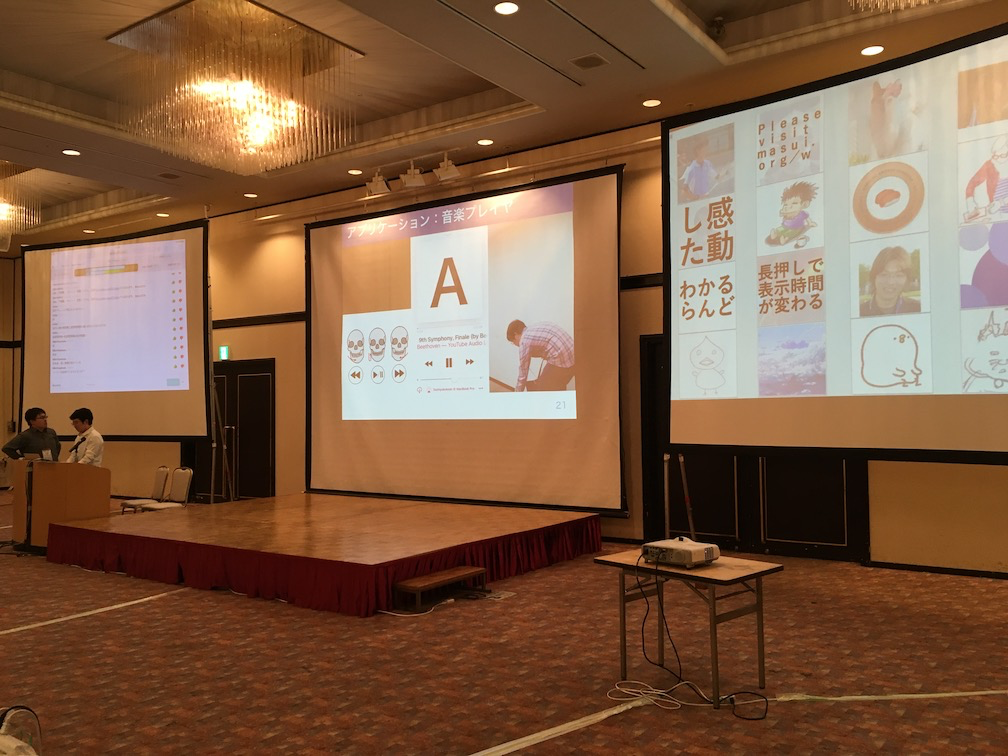
\includegraphics[width=11cm]{images/wiss2016.png}
\caption{WISS2016会場のスクリーン}
\label{wiss2016}
\end{figure}

\begin{figure}[H]
\centering
\fbox{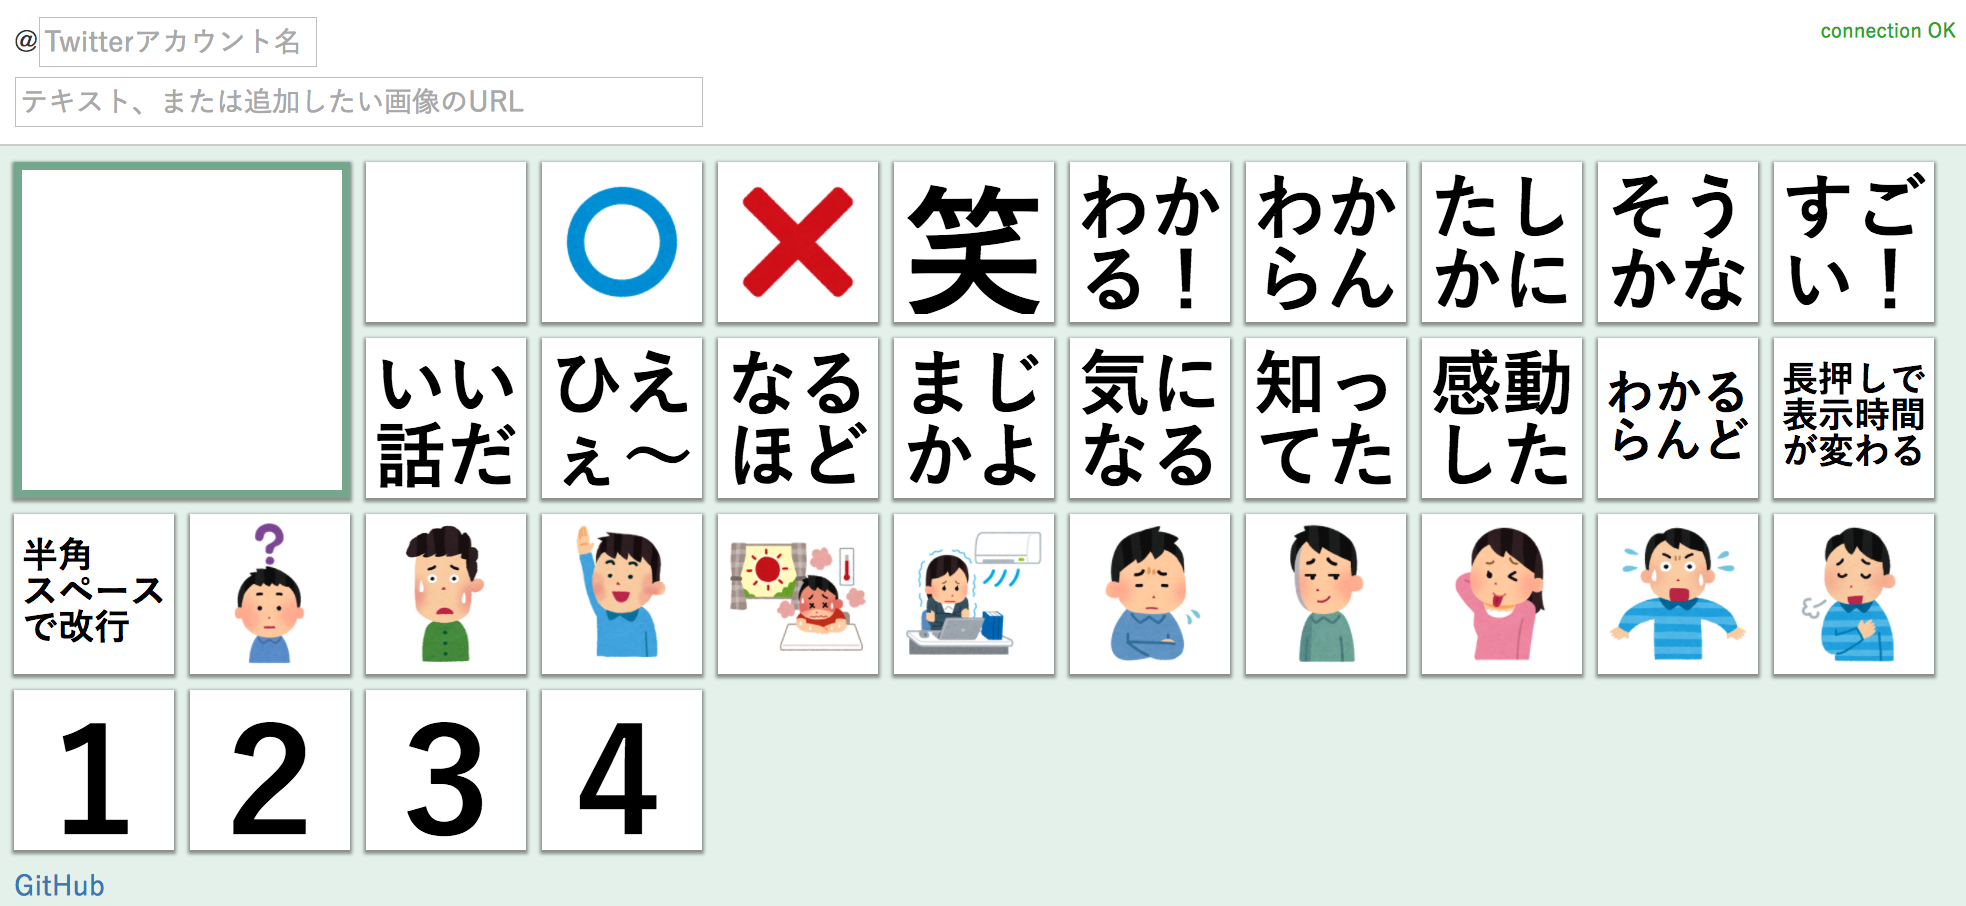
\includegraphics[width=9cm]{images/wiss2016stamp.png}}
\caption{WISS2016の『わかるらんど』でデフォルト用意したスタンプ}
\label{wiss2016stamp}
\end{figure}


\subsection{実験の評価指針}
WISSではこれまでにもさまざまなコミュニケーションシステムが運用されてきた。
しかし、各システムの運用成果報告は一部参加者のコメントを掲載するだけであったり、
システムの各機能が実際にどのように使われたかを観察した結果をまとめたものであったりするなど、
コミュニケーションシステムの定量的な評価手法は確立されていない\cite{nishida2006}\cite{nishida2011}。

今回の運用では、今までWISSで運用されてきたコミュニケーションシステムの運用成果報告と同じく、
『わかるらんど』がどのように利用されたのかを観察した結果をまとめるのに加えて、
定量的な評価としてOn-Air Forumと『わかるらんど』の投稿数を比較した。
学術会議には幅広い年齢層・背景の人が参加するため、
親しい者同士のコミュニケーションよりも精神的な敷居が高くなる。
第3章で述べたように『わかるらんど』のコミュニケーションシステムとしての設計指針は
アウトプットを増やすことであり、
アウトプットと同義である投稿の数を増やすことは本システムの評価に極めて重要である。

\subsection{実験結果}
今回が初めての実験であり過去の実験との比較ができないため、
実験結果は第\ref{chap:wakaruland}章で説明した各機能がどのように使われたのかを観察した結果を中心にまとめる。

表\ref{tb:wiss2016experiment}はWISS2016における『わかるらんど』とOn-Air Forumの運用結果である。

\begin{table}[H]
  \begin{center}
    \caption{WISS2016における『わかるらんど』とOn-Air Forumの運用結果}
    \label{tb:wiss2016experiment}
    \begin{tabular}{|l||r|r|r|} \hline
      システム & 利用人数 & 総投稿数 & 1分あたりの投稿回数 \\ \hline \hline
      わかるらんど & 71人 & 3,781回 & 5.29回 \\ \hline
      On-Air Forum & 99人 & 2,604回 & 3.64回 \\ \hline
    \end{tabular}
  \end{center}
\end{table}

3日間の会期中に全参加者の半分弱にあたる71人が『わかるらんど』で1回以上投稿した。
総投稿数は3,781回で、平均で1分あたり5.29回の投稿があった。

On-Air Forumは全参加者の約6割にあたる99人がログインし、1回以上発言した。
総投稿数は2,604回で、平均で1分あたり3.64回の投稿があった。
ちなみに、前年のWISS2015のOn-Air Forumへの総投稿数は2,948回だった。

これらの結果から、『わかるらんど』の総投稿数はOn-Air Forumの総投稿数よりも多く、
例年On-Air Forumを利用していた人の一部が『わかるらんど』に流れたことを考慮したとしても、
参加者のアウトプットを増やすという要件は満たすことができたといえる。

ユーザごとの発言数を分析すると、『わかるらんど』への投稿の約80\%は
投稿数上位約25\%にあたる18人によって行われており、概ね冪分布になっている。
また、On-Air Forumについても投稿の約80\%は投稿数上位約26\%にあたる26人による投稿で、
同じく冪分布となっていた。
図\ref{wiss2016compare}は『わかるらんど』とOn-Air Forumへの投稿数を対数グラフにプロットしたものである。

\begin{figure}[H]
\centering
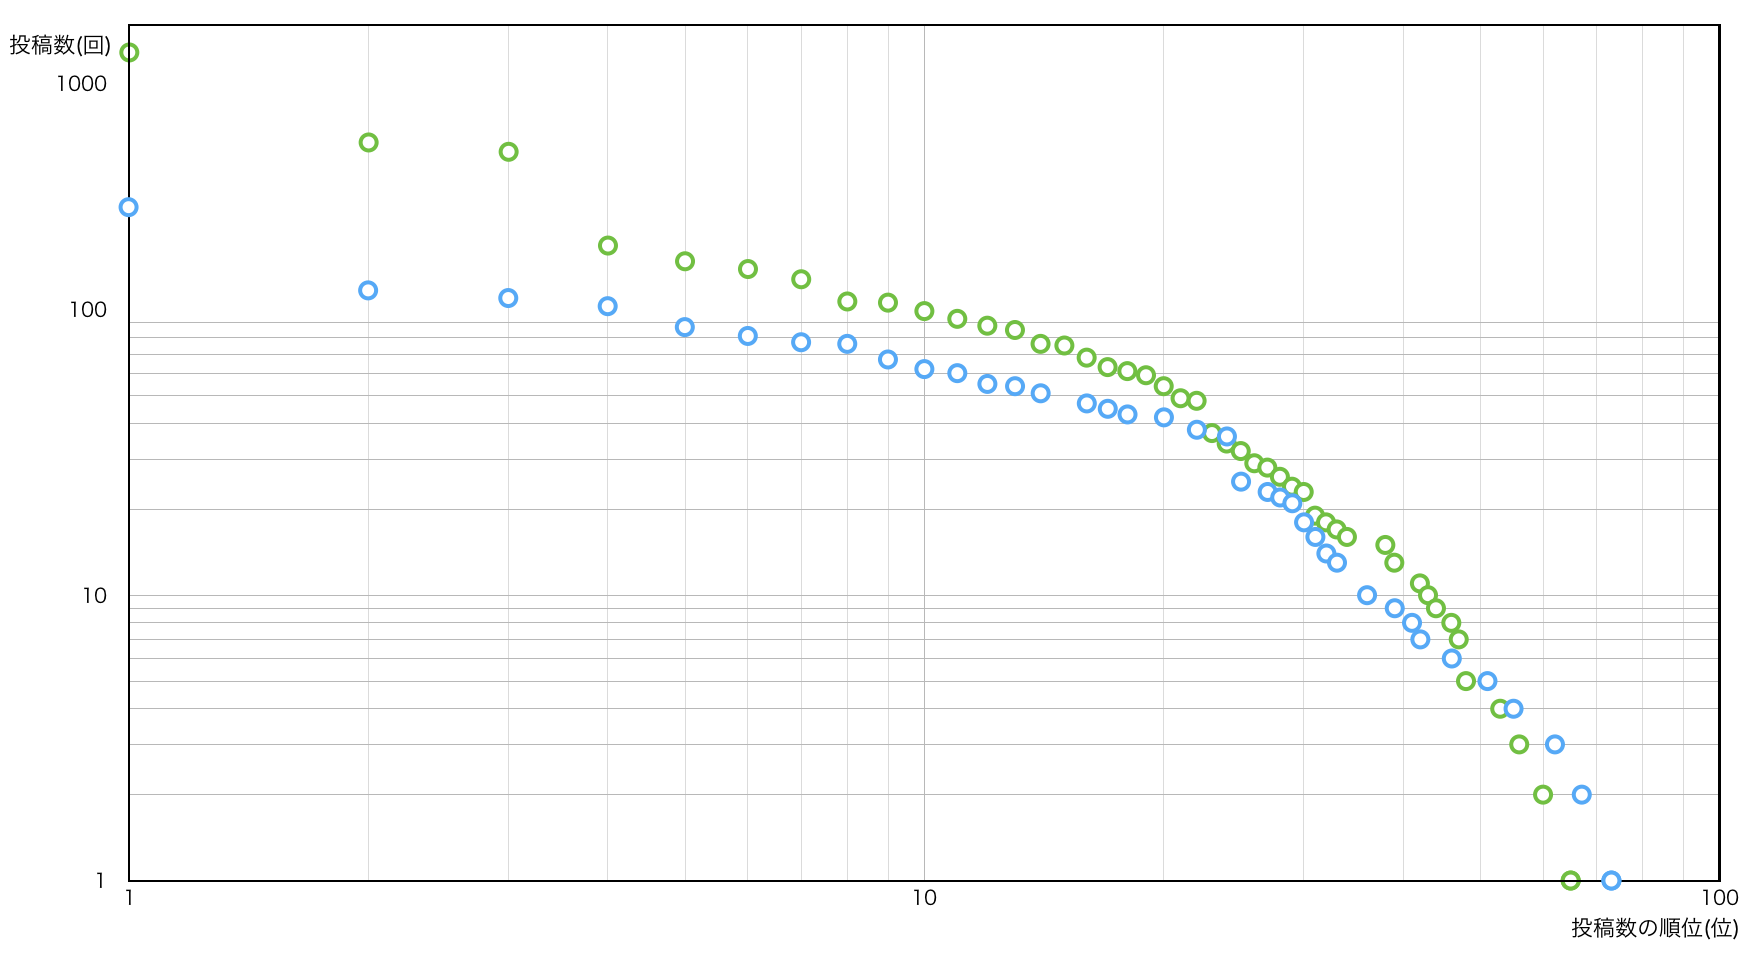
\includegraphics[width=12cm]{images/wiss2016compare.png}
\caption{WISS2016における『わかるらんど』(緑)とOn-Air Forum(青)への投稿のアカウントと発言数の分布}
\label{wiss2016compare}
\end{figure}

さらに詳細な検討によると、会の開始から会期の半分にあたる2日目の午前中までの
『わかるらんど』への参加者は41人、投稿数は1,282回であったのに対し、
2日目の午後から3日目の会期終了までの参加者は71人、投稿数は2,499回であった。
これは、参加者が『わかるらんど』の使い方に慣れてきたのに加えて、
2日目の午後から適用したアカウント名を隠した匿名化が参加者と投稿数の増加に大きく影響したと思われる。

スタンプについては、デフォルトで用意した33種類に加えて525種類のスタンプが作成され、
会期中に投稿されたスタンプは558種類であった。
最も多く使われたスタンプは「笑」で合計で141回投稿された。
2番目に多く使われたスタンプは「拍手の絵文字」、
3番目は「なる ほど」であった(表\ref{tb:wiss2016stamp})(図\ref{wiss_top3})。
「笑」は発表者が取りに行った時や、
予想だにしないアクシデントがあった時などに使用されていた。
「拍手の絵文字」は発表が終わった時に発表者に対して拍手をするタイミングで投稿されていた。
「なる ほど」は汎用性の高い相槌として、発表中に満遍なく使用されていた。

\begin{table}[H]
  \begin{center}
    \caption{WISS2016の『わかるらんど』で100回以上投稿されたスタンプ}
    \label{tb:wiss2016stamp}
    \begin{tabular}{|l|r|} \hline
      スタンプ     & 投稿回数 \\ \hline \hline
      笑           & 141回 \\ \hline
      拍手の絵文字 & 139回 \\ \hline
      なる ほど    & 114回 \\ \hline
      すご い!    & 104回 \\ \hline
    \end{tabular}
  \end{center}
\end{table}

\begin{figure}[H]
\centering
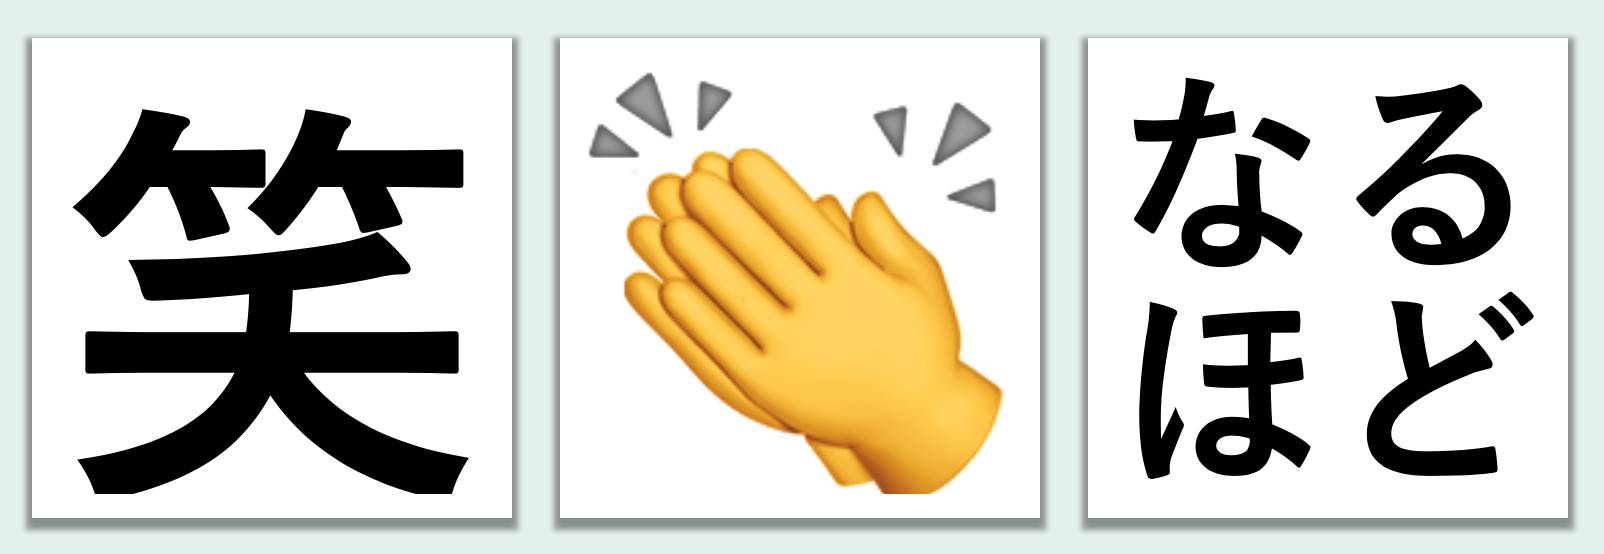
\includegraphics[width=12cm]{images/wiss_top3.png}
\caption{「笑」(左)、拍手の絵文字(中)、「なる ほど」(右)スタンプ}
\label{wiss_top3}
\end{figure}

特徴的な使われ方としては、発表中に「ポケモンGo\footnote{http://www.pokemongo.jp}」の話題が出た時や
「自由形状の竹とんぼのインタラクティブデザインシステム」の発表では、
モンスターボール\footnote{ポケモンを捕獲するためのアイテム}のスタンプ(図\ref{pokemon})や
竹トンボを飛ばす少年のスタンプ(図\ref{taketombo})
などを誰かが『わかるらんど』に投稿し、他の多くの参加者がそのスタンプをコピーして使用する
という使われ方が見られた。

\begin{figure}[H]
\centering
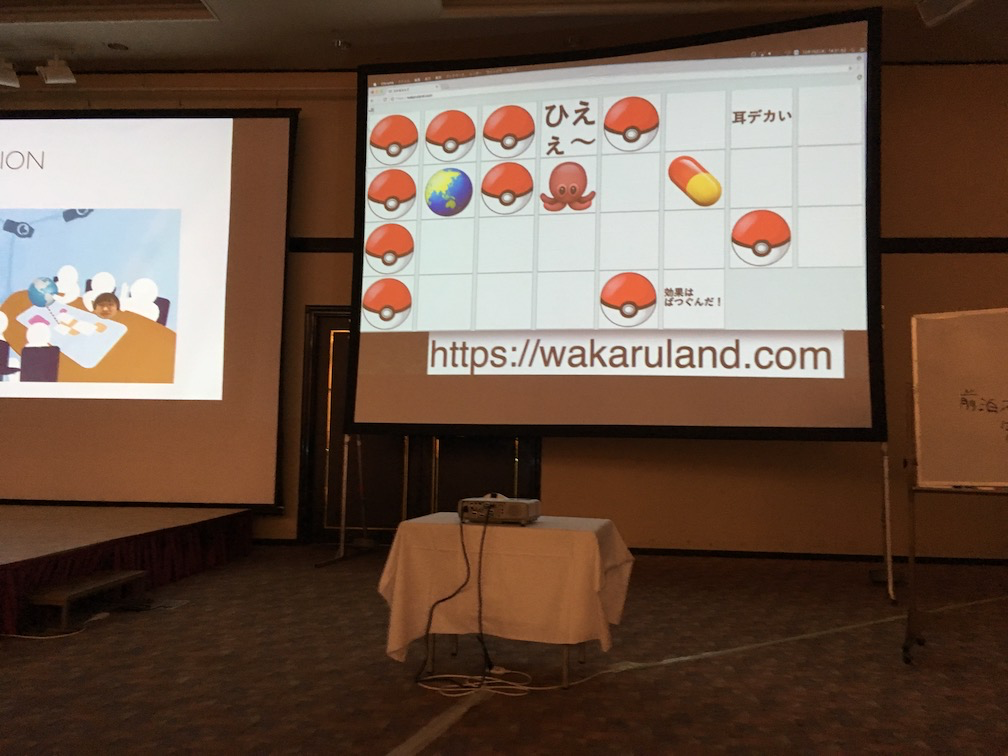
\includegraphics[width=11cm]{images/pokemon.png}
\caption{多くの参加者が『わかるらんど』にモンスターボールのスタンプを投稿する様子}
\label{pokemon}
\end{figure}

\begin{figure}[H]
\centering
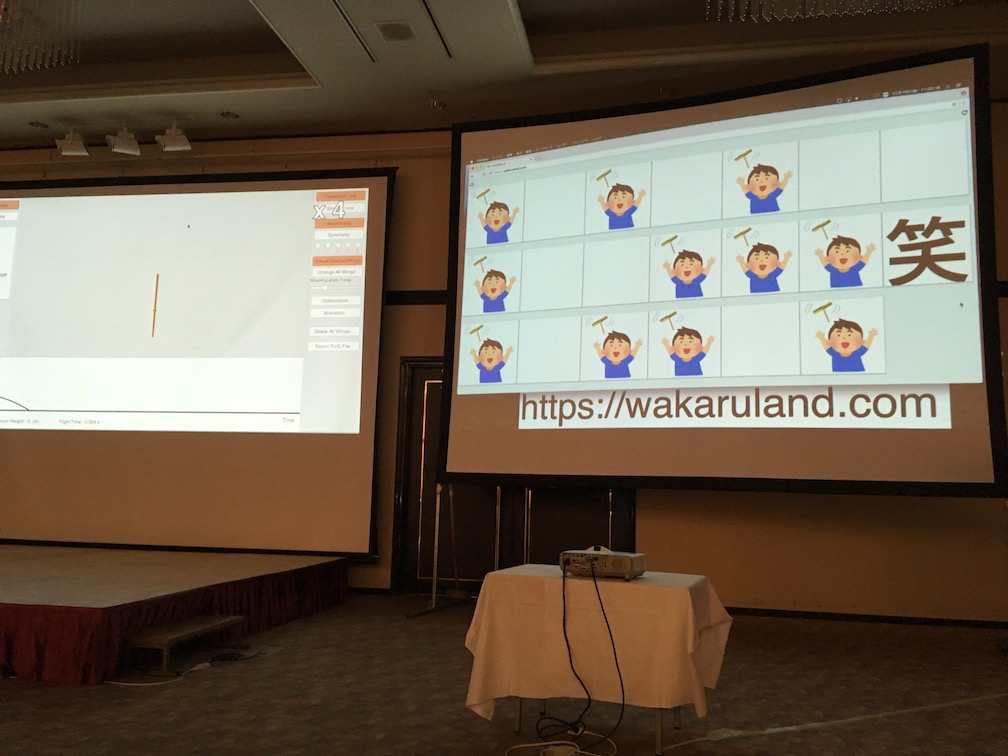
\includegraphics[width=11cm]{images/taketombo.png}
\caption{多くの参加者が『わかるらんど』に竹とんぼを飛ばす少年のスタンプを投稿する様子}
\label{taketombo}
\end{figure}


\section{研究室においての利用}
筆者の研究室では,
約9ヶ月の間『わかるらんど』を研究室内の大型ディスプレイに表示して実際に利用してきた.
筆者の研究室ではWebLindaを使用して,
Web情報やArduinoやRaspberry Piに接続したセンサ情報を利用し,
\begin{itemize}
\item 部屋の明るさを知る
\item 部屋の温度を知る
\item 風速と風向を知る
\item 入口のドアの鍵を開ける
\item 部屋の照明を点ける/消す
\end{itemize}
といったことをSlack\footnote{https://slack.com}のチャットボットを通じて行える
IoT環境を構築している(図\ref{slack})が,『わかるらんど』と組み合わせることで
さらに便利に使うことができた.

\begin{figure}[H]
\centering
\fbox{
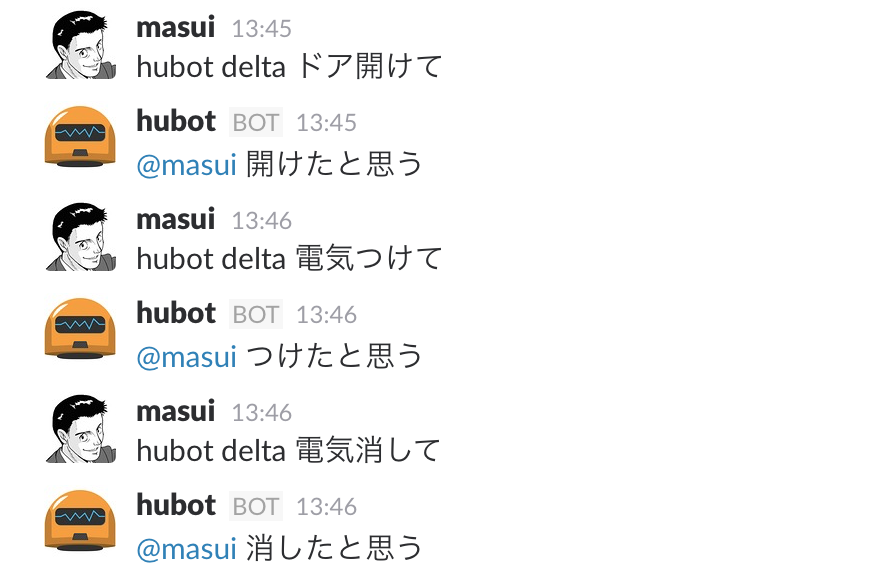
\includegraphics[width=9cm]{images/slack.png}
}
\caption{SlackのチャットボットによるIoT機器の操作}
\label{slack}
\end{figure}

図\ref{light}は部屋の明るさを表示するデータセルだが,
明るさのデータの値が小さい時は\texttt{background}画像を変更することで,
照明が点いているのか消えているのかがわかるようになった.

\begin{figure}[H]
\centering
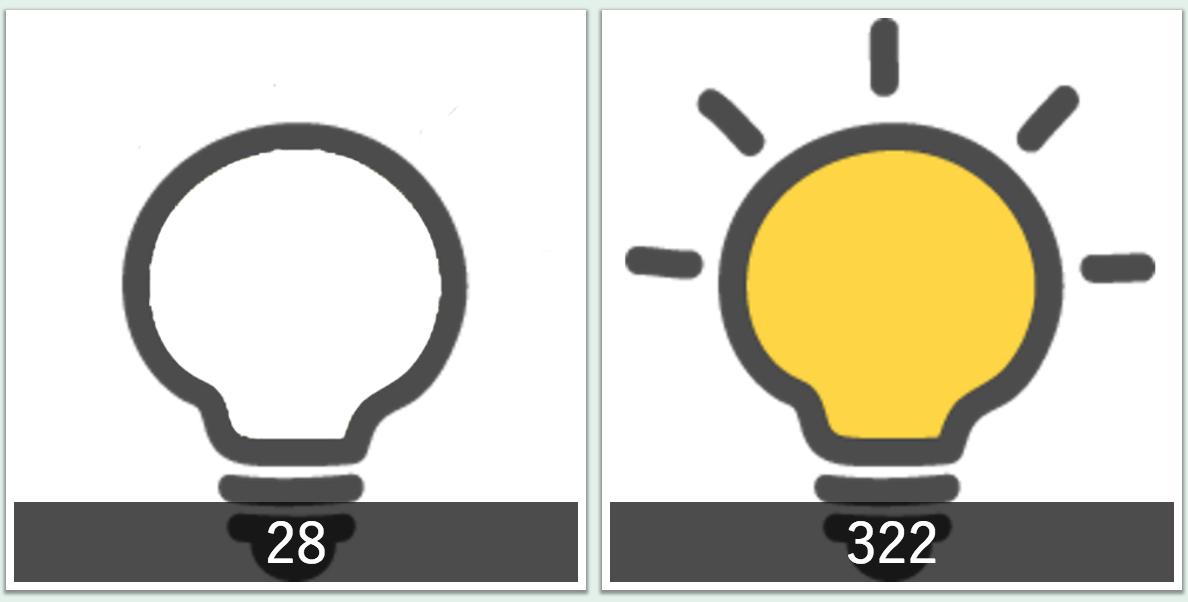
\includegraphics[width=9cm]{images/light.png}
\caption{照明が消えている時(左)と点いている時(右)}
\label{light}
\end{figure}

図\ref{door}は,研究室のドアが最後に開いた時間を表示するデータセルである.
普段は扉の画像を\texttt{background}にしているが,
実際に扉が開いた時に10秒間だけ\texttt{background}を図\ref{door}右のように
扉を開ける人の画像にすることで,誰かが入室したことが視覚的にわかるようになった.

\begin{figure}[H]
\centering
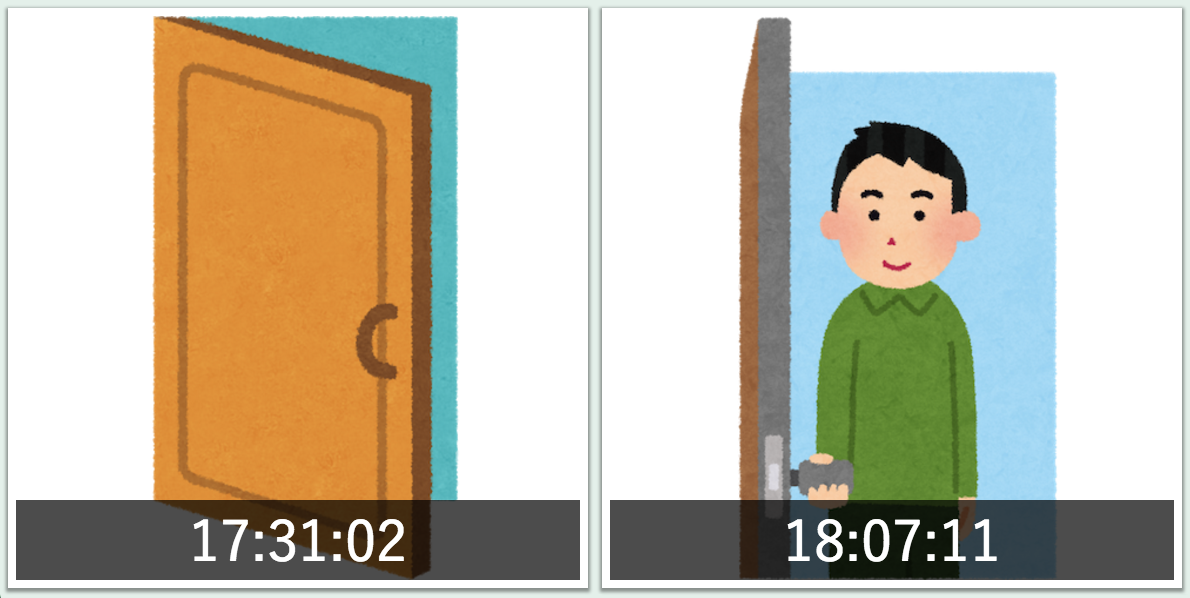
\includegraphics[width=9cm]{images/door.png}
\caption{ドアの普段の表示(左)と誰かが入室した時(右)}
\label{door}
\end{figure}

ミーティングの時間には積極的に『わかるらんど』を利用し,
普段発言の少ない人でも何らかの反応を表明したり,
発表者が聴衆の反応をひと目で把握することができるようになった.
発表中に『わかるらんど』に「わからん」というリアクションが並んだときは,
発表者が詳しい説明をすることができたり,
誰かが面白いことを言ったときに「笑」というリアクションが並び,
『わかるらんど』を通じて一体感が生まれたりすることもあった(図\ref{wara}).

\begin{figure}[H]
\centering
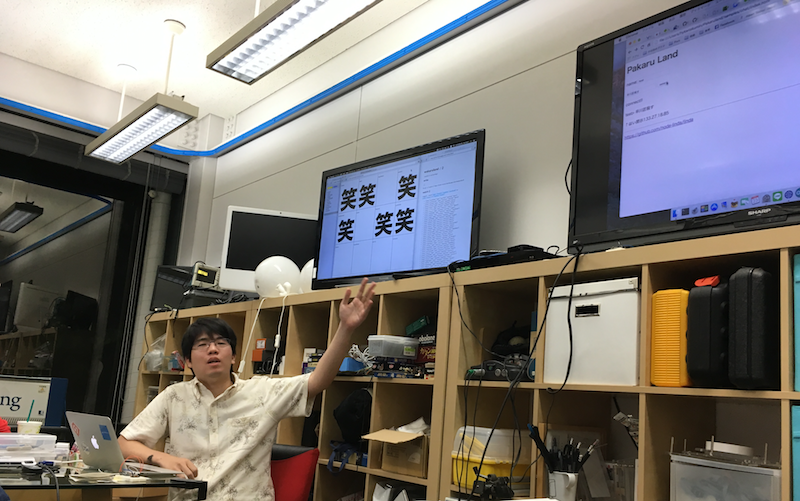
\includegraphics[width=9cm]{images/wara.png}
\caption{『わかるらんど』を使用したミーティング}
\label{wara}
\end{figure}

また,コンピュータで何か別の作業をしているときに,
Webブラウザで『わかるらんど』を開いてリアクションするのが面倒であるという意見もあった.
そこで,図\ref{heebutton}や図\ref{10key}のような
独自の『わかるらんど』入力ハードウェアを作成した.
これらを利用することで,限られたリアクションではあるが,
Webブラウザを開くことなく『わかるらんど』にリアクションを表示することができるようになった.

\begin{figure}[H]
\centering
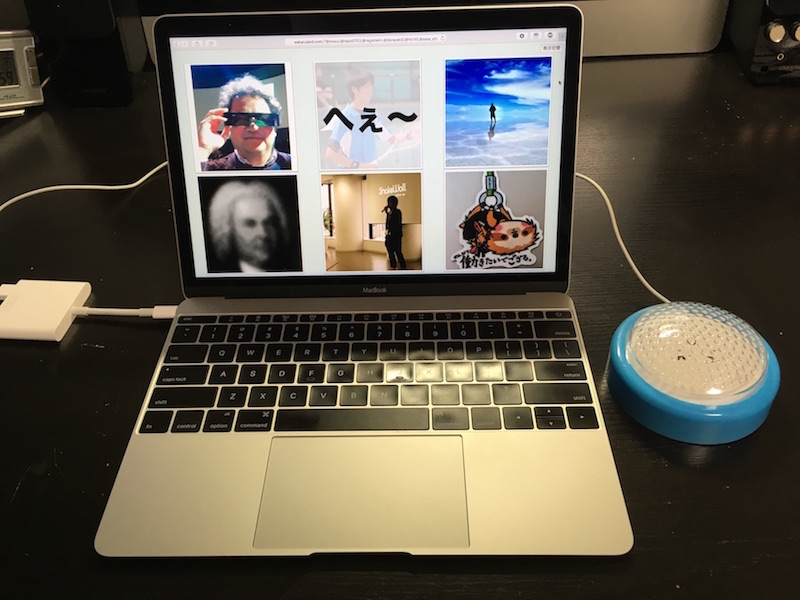
\includegraphics[width=8cm]{images/heebutton.png}
\caption{押すと「へぇ〜」とリアクションできるボタン}
\label{heebutton}
\end{figure}

\begin{figure}[H]
\centering
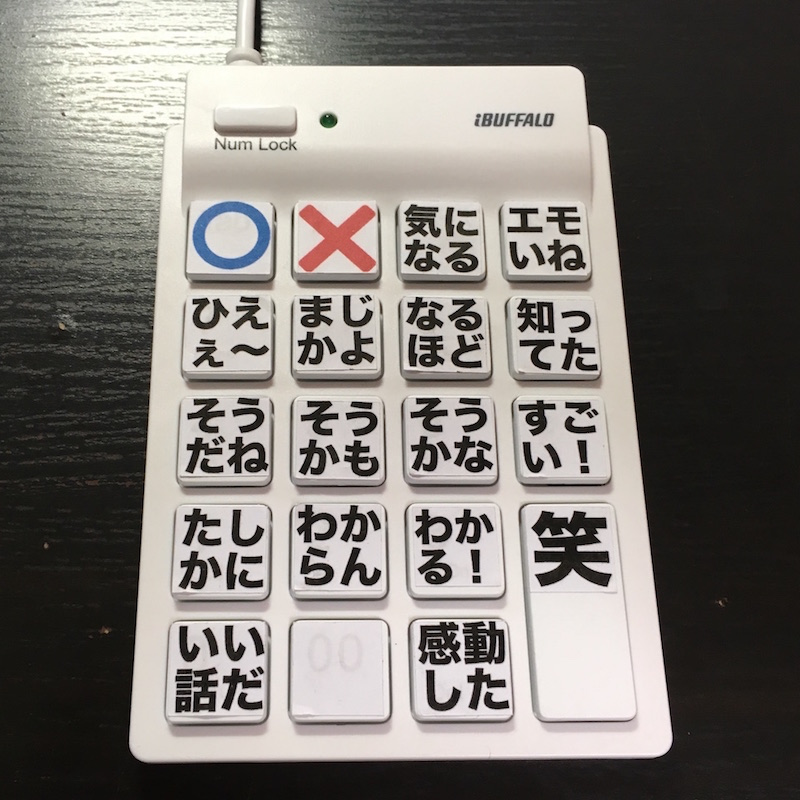
\includegraphics[width=7cm]{images/10key.png}
\caption{テンキーを利用した入力装置}
\label{10key}
\end{figure}
\chapter{議論}
\label{chap:discussion}

本章では、第6章での結果をもとに、『わかるらんど』システムの有効性と意義について議論を行う。

\newpage
\chapter{議論}
\label{chap:discussion}

本章では、本論文のまとめと結論を述べる。

\newpage



\begin{acknowledgment}

5年間の長きに渡りご指導を賜りました増井俊之教授にこの場をお借りして感謝の意を表させていただきます。



また、WISS2016において『わかるらんど』を利用してくださった皆様、
『わかるらんど』を運用する機会を与えてくださった運営の皆様に感謝します。

\end{acknowledgment}
  % 謝辞。要独自コマンド、include先参照のこと

\begin{bib}[100]
% BibTeXを使う場合
\bibliography{main}

%\begin{thebibliography}{#1}
%
%  \bibitem{参照用名称}
%    著者名: 
%    \newblock 文献名,
%    \newblock 書誌情報,出版年.
%
% \bibitem{hoge09}
%   ほげ山太郎,ほげ山次郎:
%   \newblock ほげほげ理論のHCI分野への応用,
%   \newblock ほげほげ学会論文誌,Vol.31,No.3,pp.194-201,2009.
% 
% \bibitem{hoge08}
%   Taro Hogeyama, Jiro Hogeyama:
%   \newblock The Theory of Hoge,
%   \newblock {\it The Proceedings of The Hoge Society}, 2008.
%	
%\end{thebibliography}

\end{bib}
  % 参考文献。要独自コマンド、include先参照のこと
\appendix
%\chapter{付録の例}

付録を無理矢理出力させるため、てきとうなことを書く。

\section{ほげ}

コマンドは本文と一緒。

\subsection{ふー}

本文と一緒。

\section{ほげほげ}

本文と一緒。

\subsection{ふーふー}

本文と一緒。
    % 付録

\end{document}
